\chapter{Learning to Prove}
\label{chapter:chapter_4}


\chapabstract{Like sudoku, but with types.}


Reflections are normally reserved for the end of a chapter, but I'm in a pensive mood so we'll shuffle things around.
This thesis was originally envisaged as a stepping stone toward an integrated approach at structural reasoning and meaning representation; a type-driven model of syntax reflected in a vector-based model of meaning.
When the plans were first laid down, such a deliverable was not just theoretically possible, but also technically relevant -- distributional semantics and word vectors were in their heyday, machine learning was rapidly taking off, parsers all of a sudden were becoming reliable, structured attention was a buzzword.
Everything seemed to point towards the imminent bloom of a new era in natural language processing, where the wisdoms of old would meet the machines of today, hinting at a bright and prosperous future for neurosymbolic and structure-aware models of semantic composition.
And things did seem to go that way, at least for a few years.
But, unbeknownst to all, the forthcoming era in the field's evolutionary history would actually turn out to also be its dumbest (yet).
The advent of data efficient ultra deep architectures -- combined with their immense potential for commercial applications and its allure to big tech -- brought large language models into the game.
These are unsophisticated, profanely over-parameterized, general purpose systems; fed unprocessed texts for weeks on end, until they learn to convincingly imitate its use.
With their sheer dumb force (and the hype surrounding it), large language models usurped the heir apparent and condemned structure-aware semantic computation to obscurity; the future of computational semantics is to be opaque, boring, steered by industry and provided as-a-service instead.
My thesis got caught in the blast of this change of power, necessitating a clear positioning in the current state of affairs, and a careful statement of purpose before we get to the the chapter's juicy content -- so here goes.

Parsing is good.
Converting raw signals intro structured representations thereof allows us to standardize their machine processing, and elevates automated reasoning away from form and into substance.
The more well-behaved the representational format chosen, the more powerful, transparent and verifiable the reasoning can be.
The less localized and problem-specific the representational format chosen, the more adaptive and better understood the reasoning can be.
On the basis of these observations, $\lambda$ calculi make for an ideal representation format.
Now choice of format aside, a formal system operating on formal representations is not prone to implicit biases, latent variables, ambiguity, inconsistency, or any of the the modern pestilences of the sort.
Erroneous outputs are the result of \textit{bad input} or \textit{bad programming}; there's always someone to blame.
Specifically in the natural language domain, advancing the conversion of text into formal representations is promoting accountable automation of textual processing, and eliminates the anthromorphic delusion of the ghost in the machine; for to imitate linguistic form is not to understand linguistic meaning.
Parsing is therefore only superficially in competition with large language models, and its seeming obsoletion is just a by-product of the ephemeral and rapidly shifting pop science trends of the artificial stupidity race.

That said, machine learning is not bad.
Shifting the focus away from the algorithm and toward the data can often be a reasonable concession in the automation of complex or labor-intensive tasks, provided that the task is not risk critical and that no intelligence is attributed to the end system.
This is especially the case if ``almost correct'' is almost as good as correct, or the problem being modeled is intractable, making an approximation the best we could really ever hope for.
But employing machine learning has to be thought of as either a shortcut or an admission of defeat, not as an end goal in itself.
In opting for a machine learning solution, one assigns more faith to a generic data cruncher in pretending to solve a problem than to oneself in designing a solution to that same problem.

Interweaving symbolic and subsymbolic reasoning is then the responsible engineer's out.
Complicated but decipherable components, rich in hierarchical or recursive structure, requiring or greatly benefiting from formal transparency are to be tackled explicitly.
Components that are laborious but uninteresting, data intensive or intractable are to be isolated and outsourced to a machine worker.
This partition promotes the expenditure of formal effort where it really is needed, while having it benefit from (rather than compete with) the high horsepower of brute force statistical machinery.
In this here context, I'm claiming that large language models should be treated not as a substitute, but as complementary to logic-based systems.
This is exactly the route we'll follow in this chapter, deviating from the original plan in going not from structures of form to vectors of meaning, but from vectors of form to structures of meaning.
Less pompously, we'll go through the hoops of designing and implementing a formally disciplined but accurate and robust wide-coverage parser, a neurosymbolic architecture aimed at substructural logics of the linear lineage, instantiated here for \NLPplus{} and trained on \AE thel.


\section{The Categorial Parser}
\label{section:parse}
A high-level conceptualization of the categorial grammar parser should make for a good starting point.
In the infancy of categorial grammars, the parser would be thought of as nothing other than a lexicon and a theorem prover: the lexicon enumerating any and all the possible type assignments for each word, the theorem prover exhaustively iterating the combinatorial space of assignments to produce all possible proofs for each possible assignment (Figure~\ref{figure:archetypical_parser}).

\begin{figure}[htbp]
	\centering
	\begin{tikzpicture}[t/.style={text height=1.5ex, text depth=.25ex, rectangle, outer sep=0pt}, node distance=10pt]
	\node[t] (w1) 			at (0, 0) {w\textsubscript{0}};
	\node[t] (wdots)		at (2, 0) {\dots};		
	\node[t] (wn) 			at (4, 0) {w\textsubscript{n}};
	\node[rectangle,draw=black, minimum width=120pt,minimum height=20pt] (lex)
						 	at (2, -1.5) {Lexicon};
	\draw[->]  (w1) -- ++ (0.6, -1);
	\draw[->] (wn) -- ++ (-0.6, -1);
	\node[t] (t1)			at (0.2, -3.2) {$\text{t}_0^0 \ | \ \text{t}_0^1 \ ... \text{t}_0^p$};
	\node[t] (tdots)		at (2, -3.2) 	  {\dots};
	\node[t] (tn)			at (3.8, -3.2) {$\text{t}_n^0 \ | \ \text{t}_n^1 \ ... \text{t}_n^q$};
	\draw[->] ($(w1) + (0.6, -2)$) -- ($(t1.north) + (0, 0.1)$);
	\draw[->] ($(wn) + (-0.6, -2)$) -- ($(tn.north) + (0, 0.1)$);
	\draw [thick,decorate,decoration={brace,aspect=0.2,amplitude=10pt,mirror}] (-0.5,-3.5) -- (4.5,-3.5) 
			node[black,xshift=-113.5pt,yshift=-0.6cm] {\footnotesize $\times$};
	\node[t] (c11)			at (1.5, -5) {$\text{t}^0_0$};
	\node[t] 				at (2.75, -5) {\dots};
	\node[t] (cn1)			at (4, -5) {$\text{t}^0_n$};
	\node[t] (c12)			at (1.5, -6) {$\text{t}^0_0$};
	\node[t] 				at (2.75, -6) {\dots};
	\node[t] (cn2)			at (4, -6) {$\text{t}^1_n$};
	\node[t] 				at (1.5, -7) {\vdots};
	\node[t] (c1k)			at (1.5, -8) {$\text{t}^p_0$};
	\node[t] 				at (2.75, -8) {\dots};
	\node[t] (cnk)			at (4, -8) {$\text{t}^q_n$};
	\draw[->, thick, rounded corners] (0.5, -4.3) -- ++ (0, -0.7) -- ++ (0.75, 0);
	\draw[->, thick, rounded corners] (0.5, -4.3) -- ++ (0, -1.7) -- ++ (0.75, 0);
	\draw[->, thick, rounded corners] (0.5, -4.3) -- ++ (0, -3.7) -- ++ (0.75, 0);
	\node[rectangle, draw=black, minimum height=120pt] (pr)
							at (7, -6.5)	{\begin{tabular}{c}Theorem\\ Prover\end{tabular}};	
	\draw[->] (cn1) ++ (0.4, 0) -- ++ (1.3, 0);
	\draw[->] (cn2) ++ (0.4, 0) -- ++ (1.3, 0);
	\draw[->] (cnk) ++ (0.4, 0) -- ++ (1.3, 0);
	\draw[->]  (cn1) ++ (4.3, -1.5) -- ++ (1, 0) node[right] {\{p\textsubscript{0}\dots p\textsubscript{k}\}};
	\end{tikzpicture}
	\caption{The archetypical categorial grammar parsing pipeline.}
	\label{figure:archetypical_parser}
\end{figure}

Obviously, this setup hits a brick wall in the sheer complexity of real human language.
As we have discussed in earlier chapters, a type system enacting a strict grammar logic is not just hard to design, but also entails a prohibitively ambiguous type lexicon.
Even if the theorem prover is perfectly optimized, the architecture will become bottlenecked at its input.
The total number of assignments to consider in a sentence increases exponentially with its length, so even a minor increase in the average number of types per lexical key will have a high impact in processing time.
At the same time, a fixed lexicon is a severely limiting factor, as it effectively forbids processing sentences containing unseen lexical entries (i.e. in cases of a \textlangle word, type\textrangle{} pair missing from the lexicon).
Relaxing the structural properties of the type system to ease lexical pressure is not a panacea either.
With the parser becoming increasingly ambiguous, more possibilities become accessible during search, and putative proofs become harder to reject.
From the implementer's perspective, lexicon and grammar are not synergistic but in conflict with one another, and a middle ground must be found for them to play together peacefully.

For the categorial program to come to fruition, these very real problems require equally real solutions.
The practitioner must often resort to tricks aimed at compressing or efficiently navigating the enormous search space.
The modern pipeline commonly outsources lexical disambiguation to a statistical component, referred to as the \textit{supertagger}.
The supertagger is tasked with ranking the possible assignments to a single key, given its context of appearance.
Assignments are ranked according to their likelihood, in turn approximated on the basis of some training data.
Depending on the quality and speed of the statistical estimator employed, the candidates returned are truncated depending on some threshold likelihood or by their count.
This (partially) sidesteps the explosive combinatorics of considering all potential assignments, setting an upper boundary to the cardinality of the parser's input.
The parser may also be sped up by allowing yet another statistical model to guide its actions anytime it hits a decision point.
As with all real solutions, perfect is unattainable; this time/space efficiency usually comes at the cost of approximation errors that translate to foregone rigidness, correctness and/or coverage.
The strategy we'll follow does not challenge this general model, but contributes some new insights to the operationalization of its components.

A foreword before we get to it: I imagine a crash course in machine learning to be redundant in the current day and age.
In any case, my intention is to help the purists make sense of what's going on, yet without obfuscating the implementation from fellow hackers.
To that end, I'll try keep the gory technical details contained and separate from the high level, abstract descriptions.
I hope the result is sensible and inclusive.

\section{Supertagging}
\label{section:supertagging}
A supertagger is a statistical model, a parametric function $f_\theta$ tasked with producing the most likely type assignment sequence $\tseq := t_0 \dots t_n$ for a given sentence $\wseq := w_0 \dots w_n$.
\begin{equation}
	f_\theta(\wseq) \approx \underset{\tseq}{\mathrm{argmax}} ~ p(\tseq \ | \wseq, \theta)
\end{equation}
To do so, it should in theory approximate the probability of a type assignment sequence conditional on the input; in other words, feeding $f_\theta$ with any element of the product space $\lexicon^k$ should implicitly produce a total order over the product space $\types^{k}$, where $\lexicon$ the set of words in the language, $\types$ the type universe, and $k$ ranging over $\mathbb{N}$.
If that looks stupidly intractable, it's because it is.
Both domain and codomain are practically infinite: regardless of what the cardinality of $\lexicon$ and $\types$ are, the number of combinations between different sequences thereof quickly exceeds our current estimates for stars in the universe as the sequence length increases.
Put simply, no amount of sample data would ever be able to overcome the problem's inherent sparsity and allow for a direct attempt at an approximation.
Therefore, in practice, some truncations and independence assumptions are necessary in how we choose to formulate the sequence-wide conditional assignment probability:
\begin{equation}\label{equation:supertag}
p(\tseq \ | \ \wseq)
\end{equation}
The decomposition of the seemingly innocuous~(\ref{equation:supertag}) will basically monopolize this section, because a choice of assumptions and truncations is a prerequisite for us to even contemplate the model's implementation.
Each choice can (and will) have a deep impact on the model's performance, most notably in phenomena inhabiting the more remote regions of the probability density function's landscape.
As a corollary, each choice will alter how suitable a model is to one single grammar depending exactly on how that landscape looks.
This last fact seems to have largely been dismissed by the broader practitioner community, who treat the problem with consistent indifference, changing the viewing lens only according to the quirks and fashions of contemporary machine learning standards.
We will shamelessly fall into the same last trap, but in our downfall we will at least be conscious of the intellectual and ideological roots the earlier chapters have established; those of revealing structure previously hidden, and paying that structure its due respect.

\subsection{A Brief History of Supertagging}
To actually perceive the structure, we must first notice its absence -- therefore (and for maintaining suspense), we will first outline the short but dense history of supertagging, and sketch out the paradigm shifts it has undergone throughout.

\subsubsection{Origins}
Supertagging (both the term and the idea) is due to the early insights of~\citet{joshi1994disambiguation}.
The two correctly pointed out that, for a strongly lexicalized grammar (in their case, a tree adjoining grammar), assigning the correct grammatic descriptor, or \textit{supertag} (in our case, a type), to each word in a sentence amounts to \textit{almost} parsing, and that even just weeding out some of the erroneous assignments significantly facilitates parsing.
Early literature was characterized by an almost single-minded attachment to localized computation, the justification being that supertagging must remain localized for it not to become ``too much like parsing''~\cite{bangalore1999supertagging}.
With the benefit of hindsight, we can see this for what it was: an attempt to justify a pragmatic consideration, and an artifact of the times, with the scene then largely dominated by window-based models.

A so-called unigram model assumes full independence between subsequent words, and (\ref{equation:supertag}) boils down to:
\begin{equation}
\prod_i^n p(t_i \ | \ w_i)
\end{equation}
where each local conditional can be estimated on the basis of corpus frequencies.
Despite competely breaking apart sequential sparsity, this formulation is not much good on its own either; rarely occurring lexical keys hardly provide sufficient data for an empirical distribution to be extracted.
As a solution, plain part of speech tags would find use as an intermediary, i.e. $w_i$ would in practice be substituted by $pos_i$, which would in turn be supplied by an external tagger.
The resulting model is, alas, too simple to find real use: the assumptions made are exceedingly naive, and lexicalization is heavily bottlenecked by the coarse and undescriptive part of speech tags; we need to do better.

Invoking Bayes' rule and factoring out the denominator has (\ref{equation:supertag}) rewrite to the proportionate quantity:
\begin{align}
\propto p(\wseq \ | \ \tseq)~ p(\tseq)
\end{align}
Extending the context to a window of size $\kappa$, allows local decisions to excert direct influence to the next $\kappa$ predictions (and thus indirectly affect all future ones).
This requires approximating the \textit{contextual probability} $p(\tseq)$ as:
\begin{equation}\label{equation:contextual_prob_jb}
p(\tseq) \approx \prod_i^n (t_i \ | \ \seq{t}{i-\kappa:i-1})
\end{equation}
Going one step further and making the assumption that the \textit{emission probability} $p(\mathbf{w}_{0:n} \ | \ \mathbf{t}_{0:n})$ is position-separable and independent allows its rewrite to:
\begin{equation}\label{equation:emission_prob_jb}
p(\mathbf{w}_{0:n} \ | \ \mathbf{t}_{0:n}) \approx \prod_i^n p(w_i \ | \ t_i)
\end{equation}
Putting (\ref{equation:contextual_prob_jb}) and (\ref{equation:emission_prob_jb}) together, we get an approximation to (\ref{equation:supertag}) that is blatantly wrong.
Despite the fact, it is also workable, in having efficiently circumvented sparsity, adequate, in having accounted for the very important axis of output-to-output interactions, and practical, in allowing a tangible implementation as a hidden Markov model.
Simple structural constraints would then be applied to filter out candidate predictions on the basis of admissibility criteria related to the shape and content of the supertag as well as the surrounding lexical context.


\subsubsection{CCGbank and the Original Sin}
The problem garnered attention and gained significant traction with the release of the CCGbank, the large size and gold standard nature of which offered an excellent test bed for molding the first generation of supertaggers.
The first incarnation of a combinatory categorial grammar supertagger was the original work of~\citet{clark2002supertagging}.
The model diverged from the implementation of~\citet{bangalore1999supertagging} in opting for a larger window size and foregoing the contextual effect of output-to-output dependencies.
In that setting, and for a window of size $2\kappa + 1$, (\ref{equation:supertag}) takes the form:
\begin{equation}
	\prod_i^n p(t_i \ | \ \seq{w}{i - \kappa : i+\kappa})
\end{equation}
The model would materialize as a log-linear feature weighter trained as a maximum entropy estimator.
The input would include several sparse heuristics, including morphological features and boolean context predicates, allowing a partial soft bypass of the fixed-key lexicon.

Novelty and ingenuity aside, the work set a number of precedents; some of those, reasonable as they may have been at the time, have since permeated through the problem statement, becoming de facto practices rather than conscious design decisions.
Structural constraints were dropped, in part because they are less straightforward to deduce in frameworks other than tree adjoining grammars; they never found their way back into the mainstream, athough admittedly they never were particularly sophisticated to begin with.
This step away from structural discipline is exacerbated by having also dropped the supertag-to-supertag dependencies, since the model now has no chance of learning how to statistically filter out mutually incompatible assignments either.
To counteract the problem, the paper opted for a yet more radical solution: abandoning the sequential formulation (i.e. no more $\mathrm{argmax}$ing over the product) in favor of a \textit{multitagging} approach (i.e. returning all categories whose local probability exceeds some fixed ratio of the highest ranked candidate).
This was shown to greatly improve coverage (by outsourcing heavier duty to the parser), but has to be understood as a practical overcorrection, an emergency measure to sidestep the model's inherent disregard for output-level sequential interactions.
The limitation is acknowledged by \citet{clark-curran-2004-importance}, and an attempt at resolution is offered by \citet{curran2006multi}.
There, the forward-backward algorithm is employed to efficiently calibrate the probability of an assignment (in the multitagging setup) as the sum of all sequential assignments containing it:
\begin{equation}
	p(t_i \ | \ \mathbf{w}_{0:n}) = \sum_{\mathbf{t}_{0:i-1}, \mathbf{t}_{i+1:n}} p(\mathbf{t}_{0:i-1}, t_i, \mathbf{t}_{i+1:n} \ | \ \mathbf{w}_{0:n})
\end{equation}
This does reinstate a notion of output-to-output dependencies in the form of estimated posteriors, but computational considerations have diffused the potential for widespread adoption in later frameworks. 
Finally, rare supertags, which were particularly problematic or near impossible to learn, were found to have very limited impact on overall coverage; this set the grounds for their statistically near-inconsequential erasure, a choice that gradually became ingrained as a mandatory step of data sanitation and preprocessing.


\subsubsection{Distributed Word Vectors \& Neural Networks}
The advent of word embeddings and the gradual substitution of sparse features with continuous vectors paved the way for the incorporation of artificial neural networks.
\citet{10.1162/tacl_a_00186} employed a collection of pretrained embeddings combined with a window-based two-layer network in a ``semi-supervised'' manner (in today's jargon, a pretty much fully supervised separable convolution), to a dual effect.
On the one hand, the pretrained embeddings offered a natural generalization from the fixed size lexicon to the (still fixed, but much larger) set of pretrained` embeddings, single handedly obsoleting the long standing problem of tackling rare and unseen words~\cite{thomforde-steedman-2011-semi,deoskar-etal-2011-learning,deoskar2014generalizing}.
On the other hand, the parameter-sharing convolution improved the accuracy/ambiguity ratio and overall efficiency of the (then standard) log-linear supertagger of~\citet{clark2007wide}.
Unlike before, words were allowed to associate to any supertag, regardless of whether or not a \textlangle word, supertag\textrangle{} pair was observed during training; the lexicon thus turning from a hard imperative to a soft guideline.
Additional experiments involving a conditional random field were mildly successful, but abandoned due to the prohibitively slow decoding -- yet, it is obvious to the people involved that something critical is missing.
\citet{xu-etal-2015-ccg} took the approach a step further by utilizing a simple recurrent network (RNN), and, in doing so, claimed to sidestep the locality of the previous neural model.
To escape the unidirectional constraint of the classical recurrent network (or perhaps out of force of habit?), they continued incorporating window-based features that provided a minimal amount of right context $\kappa$, thereby rewriting (\ref{equation:supertag}) as:
\begin{equation}
	\prod_i^n p(t_i \ | \ \seq{w}{0:i+\kappa})
\end{equation}
And while their approach does indeed offer a wider receptive field, it is focused solely on the input side; output-to-output interactions are still nowhere to be seen.

\subsubsection{Autoregressive Modeling}
By now (and despite earlier aphorisms), it is becoming increasingly evident that nothing deep or spiritual restricts supertagging to remaining local, as advancements in machine learning are progressively offering more opportunities for fast and efficient incorporation of ever wider context.
But the absence of output-to-output dependencies remains unresolved, despite them being a recurrent theme in the literature.
This changes with the work of \citet{vaswani-etal-2016-supertagging} who score two major points with their resourceful use of long short-term memory networks (LSTM).
First, they replace the simple recurrence of \citet{xu-etal-2015-ccg} with a bidirectional one (thus allowing unbounded left- and right- input interactions) --  an idea explored in parallel by multiple contemporary works~\cite[inter alia]{ling-etal-2015-finding,xu-etal-2016-expected,lewis-etal-2016-lstm}.
More importantly and in addition to that, they introduce an intermediate recurrence that is to serve as a supertag-level language model, fusing the prediction history with the input context to produce each local prediction.
The two together alter (\ref{equation:supertag}) into a version far more elaborate than previous proposals:
\begin{equation}\label{equation:lstm_lm}
	\prod_i^n p(t_i \ | \ \seq{t}{0:i-1},\wseq)
\end{equation}
Under a modern lens, this is akin to a somewhat idiosyncratic implementation of an autoregressive sequence-to-sequence model, with the decoder benefiting from perfect alignment between input and output tokens.
Unlike prior work, no occurrence threshold was imposed, and explicit evaluations over sparse lexical relations were provided.
The added expressivity and significantly wider receptive field granted LSTM models the state of the art badge, which was to remain uncontested for a surprisingly long two human years%
	\footnote{Approx. three centuries in machine learning years.}.

\subsubsection{Superwhat?}
More than just a testament to the LSTM's strengths, this momentary pause makes for a discontinuity in the velocity of progress; not because people suddenly lost interest in supertagging, but rather because machine learning architectures and their applications had slowly become exhausted.
This coincides with a stall across NLP in general, and a concurrent paradigm shift; specialized models started becoming outfashioned, and improvements would no longer be enabled by domain expertise and task-specific engineering, but rather by higher quality unsupervised and semi-supervised training routines over larger and larger models.
A case in point is the next major landmark, in fact reached by a structurally simplified model~\cite{clark-etal-2018-semi}, 
a plain bidirectional sequence encoder using the factorization:
\begin{equation}\label{equation:seq_cls}
	\prod_i^n p(t_i \ | \ \wseq)
\end{equation}
Despite taking a step backwards in terms of structural sophistication, the model managed a performance leap comparable to that of switching from a separable neural function to a recurrent one (see Figure~\ref{figure:supertag_history}), all by ``simply'' incorporating multiple tasks and losses in its training loop.
The same paradigm is today more dominant than ever, and has pushed conventional NLP outside of the spotlight, putting an end to an exciting but short golden era.

\begin{figure}
	\centering
	\begin{tikzpicture}
	\begin{axis}[
	    xlabel={Publication Year},
	    ylabel={Accuracy (greedy)},
%	    xmin=1, xmax=48,
%	    ymin=-0, ymax=1,
%	    xtick={1,10,100,1000,10000, 100000}, 
	    legend pos=north west,
	    ymajorgrids=true,
		minor y tick num=1,
	    yminorgrids=true,
	    xmajorgrids=false,
%	    xminorgrids=true,
	    axis line style={draw=none},
	    tick style={draw=none},
%        legend pos=north east,
		xticklabels={,,2002,,,,,,,,2018},
		x tick label style={/pgf/number format/.cd, 1000 sep={},},
        width=0.85\textwidth,
		enlarge x limits=0.1,
		point meta=explicit symbolic,
		nodes near coords,
         nodes near coords style={
         	anchor=west,
            font=\small,
        },
	]
	    
	 
 	\addplot[mark = *, only marks,mark options={black}]%]
 		table[x=X,y=Y,meta=M] {
 			X		Y		M
 			2002 	90.5 	\citet{clark2002supertagging}
 			2004	91.5	\citet{clark-curran-2004-importance}
 			2014	91.3	\citet{10.1162/tacl_a_00186}
 			2015	93.07	\citet{xu-etal-2015-ccg}
 			2016	94.24	\citet{vaswani-etal-2016-supertagging}
 			2016	94.7	\citet{lewis-etal-2016-lstm}
 			2018	96.05	\citet{clark-etal-2018-semi}
 		};
	 \end{axis}
	\end{tikzpicture}
	\caption{Supertagging performance in the CCGbank historically.}
	\label{figure:supertag_history}
\end{figure}


\subsection{Constructing Types}
The supertagging architectures reviewed are, from first to last, variations on a theme.
Regardless of whether the underlying statistical machinery is a hidden Markov model, a maximum entropy model, a neural sequence tagger or a sequence-to-sequence transducer, a single commonality characterizes them all: they start from the assumption of a finite codomain.
More than that, they don't just assume but \textit{require} that the zipfian tail of lexical type sparsity is practically irrelevant for the corpus, and, by extension, for language at large.
In other words, they require that most of the probability mass of type occurrences is concentrated around a central region of a few common types, and that exceptionally rare types are nothing but statistical artifacts which can safely be ignored.
This bias is not to be mistaken for a vice, nor for a deeply motivated ruling; it is a practical compromise that became an unwritten rule, similar to the (once proclaimed as necessary) locality of supertagging -- a notion since abandoned and forgotten with minimal remorse and deliberation as soon as technology allowed.
The issue is really quite shallow: statistical models have always had a very hard time dealing with under-represented samples (in our case, supertags), and correctly recognizing items outside the training data is an open problem with no general solution.

That is not to say the compromise is an unjust one; its heedless proliferation does come with two major side effects, though.
One, it forces parsers to give up on potentially rare syntactic phenomena, assuming those manifest through unique and uncommon supertags.
Even though a parser should in principle be able to handle any valid supertag (regardless of its statistical properties), the a priori exclusion of rare ones corresponds to an externally imposed restriction to its generalization.
In other words, exactly those difficult phenomena that would benefit from the linguistic expertise of a robust parser are to be discarded in the first place!
There's a bit of a self-fulfilling defeatism here: we'll always only parse what we \textit{can} parse, sure, but we'll never be able to parse what we won't ever \textit{try} to parse.
Two, in becoming part of the first page of the (as of yet unwritten) supertagging bible, the concept implicitly reinforces the belief that grammars not following a distribution of occurrences similar to (or denser than) that of the CCGbank are practically unusable.
A densely featured type system and its overpopulated lexicon have become demonified as pitfalls we have to steer away from, which is actually quite the contradiction -- we came up with supertagging to treat lexicalized grammars, but we won't push lexicalized grammars further because of a lingering fear that our supertaggers are not good enough, i.e. lexicalization is good, but only as long as it's not too lexicalized! 

Epistemological ramblings aside and back to reality, the type grammar we have developed is not among the lucky few.
\AE thel is way sparser than the CCGbank, containing five times as many types, while test samples with at least one rare type (i.e. a type with less than 10 occurrences in the joined train and dev subsets) appear four times as often as in the CCGbank (14.5\% vs 3.5\%).
Disregarding rare types is making ourselves content with an idealized (unachievable) peak sentential parsing accuracy of 86.5\%, which is far from an aspiring start.
Worse yet, these statistics are suggestive of a big type universe%
	\footnote{Read as (big (type universe)) and not as ((big type) universe) -- if you don't see the difference, ignore this comment.}, 
of which we likely have a observed only but a glimpse through the lens of \AE thel.
In practical terms, we done messed up, and no existing technology will save us now.
But, as the proverb goes, ``necessity is the mother of invention'' and we're definitely in need here, so we may as well invent something.

In reality, what we need is less of an invention and more of an observation.
The important thing to observe is that supertags (be them combinatorial categories, type-logical types or anything resembling them) are not ad hoc, opaque and dissimilar \textit{units}, but highly regular, transparent and decomposable \textit{structures}, made of a small set of primitives and the operations that piece them together.
In our setup, complex types are the result of type forming operators applied to ``smaller'' types, the smallest types available being atomic propositions; recall the (strategically placed) exercise of Figure~\ref{figure:litten_acg_der}.
This insight is not a particularly deep one; it won't come as a surprise to anyone that has even superficially dabbled in the joys of algebraic data types, context-free grammars, inductive tree structures, or any sort of the hierarchical recursions common in computer science.
Theoretically unsurprising as it may be, it offers an interesting applied perspective: why teach a statistical model how to \textit{disambiguate} (i.e. choose) between some candidate assignments (however many), when we could instead teach it to \textit{construct} (i.e. inductively describe) the most suitable assignments instead?
A system able to consult the present linguistic context in order to construct well-formed and well-motivated types would amount to the first ever specimen of a new species: a supertagger with an unrestricted codomain.
We'll call this species of supertaggers \textit{constructive}.
This perspective is in a sense orthogonal to the transition from fixed, corpus-extracted assignment frequencies to word vectors. Whereas one generalizes over rare and unseen items in the first coordinate of lexical entries (\textlangle word, type\textrangle{} pairs), the other does so over the second.
The two, combined, lift the closed world assumption, paving the way for the last supertagger we'll ever need -- one able to reliably predict the correct type (be it rare or unseen) for any word (be it rare or unseen).

\subsection{Supertagging as NMT}
\label{subsection:snmt}
The first attempt at a constructive supertagger is described in detail by~\citet{kogkalidis-etal-2019-constructive}.
Like all first attempts, it is characterized by a degree of cute naivety combined with an overeager execution.
Types are first viewed as the corresponding formula trees, and then traversed in a depth-first left-first fashion (i.e. read off in Polish notation).
Each type thus yields a type-word, viewed as the produce of a tiny recursive grammar (a context free one), the alphabet of which would be the union of propositional constants and logical connectives.
A sequence of types is represented as the concatenation of the sequentialized types, each type-word separated from the next by an (in hindsight unecessary) special alphabet token.
This expansion of a type-word into multiple symbols inadvertently breaks the input-to-output alignment; words are no longer associated to a single output symbol, but rather a sequence thereof.
As expected, this means that a sequence tagger is no longer a fitting backend for our experimental ventures.
Thankfully, the two biggest buzzwords of machine learning in 2018 are both surprisingly relevant here.

\subsubsection{Buzzwords}
\paragraph{Neural Machine Translation} Neural machine translation (NMT) is the modern paradigm to machine translation, the task of automatically translating text from some source language to a target one.
The term made its explosive first appearance halfway through the last decade, taking the field by storm~\cite{kalchbrenner2013recurrent,cho2014learning,bahdanau2015neural}.
The dominant approach rests on a sequence-to-sequence neural model~\cite{cho2014learning,NIPS2014_a14ac55a}, which consists of two parts: a sequence \textit{encoder}, which builds a contextual representation of the input sequence, and a sequence \textit{decoder} which uses the input representation to iteratively produce the output sequence on a token by token basis.
For an input sequence $\seq{x}{0:M}$ mapped to an output sequence $\seq{y}{0:N}$, this corresponds to a conditional language model trained to maximize
\begin{equation}
	p(y_i \ | \ \seq{y}{0:i-1},\seq{x}{0:M})
\end{equation}

The above conditional is identical to (\ref{equation:lstm_lm}); in fact the supertag language model of~\citet{vaswani-etal-2016-supertagging} \textit{is} a degenerate case of neural machine translation, where $\mathbf{y}$ is $\mathbf{t}$ and $\mathbf{x}$ is $\mathbf{w}$, and $M$ and $N$ coincide.
This is not a one-off, but rather an instace of a broader trend, referred to as \textit{generalized} machine translation.
The generalized part stems from the fact that neither the source nor the target language are in any way constrained to being natural (or human) languages; either of the two (or both!) may well be artificial languages.
The actually interesting bit is that they don't actually even need to be languages \textit{per se}; any complex data structure that can be canonically traversed into an unambiguous sequentialization makes for a valid input/output.
\citet{vinyals2015grammar} explore the idea in training a sequence-to-sequene parser by directly translating the input sentence into a linearized constituency tree; the model is surprisingly accurate in learning both \textit{how} to create valid trees (only occasionally producing malformed output), and \textit{which} valid tree to create for a given sentence (with an accuracy comparable or matching previous established models).

The paradigm per se is rather bland, making no assumptions about the output structure and requiring little to no task-specific tuning.
For the exact same reasons, it is also highly appealing, and a good starting point for experimentation -- we can just apply it virtually unchanged to the task at hand.
In our domain, the goal sequence $\mathbf{y}$ would be the sum of symbols together forming our sequence of type-words, and $\mathbf{x}$ will be none other than the sentence itself.
Using the doubly indexed $s_{i,j}$ to denote the $j$-th symbol of the $i$-th type (symbol enumeration following the depth-first left-first traversal of the formula tree), the conditional becomes:
\begin{equation}
	\prod_i^n \prod_j^{|| t_i ||} 
	p(s_{i, j} \ | \ 
		s_{k, :} : k < i,
		s_{i, k} : k < j,
		\wseq)
\end{equation}
where $||t_i||$ the number of symbols of type-word $i$.
We will refer to this operationalization as a \textit{symbol sequential} supertagger.
Note that the above is essentially an expanded version of~(\ref{equation:lstm_lm}), in the sense of containing intermediate evaluations in between full supertags.
This view allows drawing a parallel between type-words made of primitive symbols and words made of subword units~\cite{sennrich-etal-2016-neural}. The two share the same high-level purpose of improving ``translation'' to rare (type-)words, even though the structural decomposition of types is much more regular and consistent than the morphological decomposition of words.

\paragraph{Neural Attention}
Encoding the input sequence to a fixed length vector is essentially lossy neural compression.
The longer the input and output sequences are, the more this compression may prove catastrophic in capturing long range dependencies~\cite{cho2014properties}.
As an alternative, attention-based models circumvent the need for compression by simply building a contextually informed representation of the full input, distributed evenly among its tokens (one representation per sequence element).
These representations can be dynamically weighted and summed, yielding a distinct view of the same structure based on an external aggregation context (a query).
Attention has its roots in neural image processing~\cite[inter alia]{larochelle2010learning,NIPS2014_09c6c378}, but its application to language was essentially the catalyst that set the field ablaze~\cite{bahdanau2015neural}.

Even though attention was originally used as an enhancement on top of RNNs, the code of conduct today is basically attention only.
The instigator of that paradigm shift was the transformer architecture~\cite{vaswani2017attention}, which by now enjoys an unprecedented pop-science status (saving me the hassle of having to regurgitate yet another ``transformers explained'' pamphlet).
In high level terms (and consciously oversimplifying), the transformer is a heteroassociative memory mechanism.
It builds three distinct representations for each sequence token: \textit{queries} dictate what each token looks for, \textit{keys} dictate what each token associates with, and \textit{values} correspond to stored memories.
A distance metric (commonly a scaled dot-product) is used to induce a weighting over the keys matrix for each query vector; we may say that queries \textit{attend} to keys.
The resulting weights are normalized to sum to one, and act as multiplicative factors in the weighted averaging of the values matrix, yielding a vector acting as a distinct evaluation of the full sequence for each query.
This basic operation is trivial to parallelize, both across tokens within the same sequence, as well as across independent sequences, thus allowing an efficient many-to-many message passing contextualization that can be stacked multiple times in depth for extra expressivity.
Using this as a decoder is just as easy, since queries may come from a different sequence than keys and values, provided their dimensionalities (not the counts!) match.
The only requirement is a masking strategy that disallows autoregressed tokens from attending to their future while training (since that would be cheating).
This is significant for training in the NMT setup, as it circumvents the linear temporal delay of the RNN by trading it for the quadratic memory cost of the attention matrix (quadratic because all tokens must attend to all tokens); the trade-off does not carry through to inference, where one has to suffer both the temporal delay (since there's no oracle supplying the future anymore) as well as the memory penalty.

\subsubsection{Implementation}
Our problem is ripe with long distance dependencies.
Moreover, these are not confined to being only between encoder-decoder token pairs, but may also occur within decoder token pairs alone.
Consider that the misalignment between input and output means that we must consult the full input sequence at each decoding step, while the structurally liberal type logic means that cues to the current step may be found locally (within the same type), or multiple types (and thus even more steps) away.
For this reason alone, the transformer seemed like a good candidate architecture.
Adhering to evidence that pretrained language models seem to benefit either side of the encoder-decoder pipeline, the encoder would consist of a Dutch version of ELMo, the de facto language model at the time~\cite{peters-etal-2018-deep,che-etal-2018-towards}.
To account for domain adaptation without having to compute the costly gradient updates for the over-parameterized language model, a single transformer encoder was used to contextualize ELMo's precomputed representations.
The encoder was connected to a tiny transformer decoder of two layers, allowing unhindered access to the full input and all previous outputs.

\subsubsection{Experiments \& Results}
\paragraph{Training}
The model was trained with teacher forcing, i.e. predicting the current step assuming perfect rather than predicted (noisy) context.
For regularization, and in order to discourage the model from memoizing common type patterns, the Kullback-Leibler divergence was employed as the loss function, computed between the model's predictions and the ground truth, with 20\% of the probability mass evenly distributed across the non-true entries (basically a naive implementation of the label smoothed cross entropy loss~\cite{szegedy2016rethinking}).
The training data would consist of samples counting less than 20 words, pulled from the version of \AE thel then current.
This historical version of the dataset diverges considerably from its present incarnation, the core difference being the use of $\NLP$ as the type logic, with an informal decoration of the implication standing for today's modalities.
Despite formal and representational divergences, the distribution of types is practically identical in between the two versions; as a fun trivia, only about 85\% of the total unique types were present in the training split used.
Modulo exact numbers, insights gained from this past venture do carry over to the present.

\paragraph{Evaluation}
Unlike work in CCGbank, evaluation cannot be done on a comparative basis, due to the absence of established baselines%
	\footnote{There's basically noone to beat.}.
Cross-framework comparisons are also irrelevant due to the vastly different problem formulations (i.e. different linguistic framework, corpus, language); to drive the point across, consider that accuracy was measured over a set of 5\,700 types, which is 1 order of magnitude above CCGbank's 425 non-thresholded categories.
What's worth exploring instead is (i) the architecture's potential at supertagging, and (ii) its ability to learn reasonable generalizations beyond its training data.
To that end, we may view constructive and discriminative supertagging not as two orthogonal approaches, but as the extreme points of a continuum.
At the intermediate points between these extremes, there exist alphabets containing composite symbols that correspond to notational shorthands for the most common type and sub-type patterns.
As more of notational shorthands are introduced, the target output's length is significantly decreased, but the model is exposed to progressively less constructions of full types.
This becomes useful in approximately mapping the landscape between a fully constructive supertagger and a fully discriminative one.

On a purely numerical basis, the results are not astounding. 
Constructive accuracy lies at a disheartening 88\%, which is far from sufficient for downstream parsing.
What is intriguing, though, is that accuracy gradually declines with the introduction of notational shorthands, falling all the way down to 87.2\% with the eventual collapse to a discriminative autoregressive tagger.
Let's repeat this once more: obfuscating type structure hinders performance.
The story looks even more promising when it comes to the far end of the zipfian tail: 19.2\% of type assignments involving unseen types are correctly predicted, as are 45.7\% of those involving rarely seen types; these plunge to an unavoidable 0 and 23.9\%, respectively, with the transition to a discriminative setup.
Furthermore, not a single type is malformed, indicating that the grammar of type formation is indeed learnable, even when incorporated within a challenging sequence labeling task.
Raw numbers aside, the results suffice to deem the experiment an objective success: we generated concrete evidence that a full dismantling of the lexicon is not just \textit{possible} but in fact also \textit{beneficial} for supertagging a sparse type grammar.

\subsubsection{Insights \& Observations}
\paragraph{Advantages}
The prime advantage is the acquisition of rare and unseen supertags, which is a major accomplishment in its own right.
Secondary advantage \#1 is the unintended provision of trained representations for zeroary and n-ary primitives%
	\footnote{Replace with appropriate framework-specific terminology, e.g. atomic propositions and logical connectives, atomic categories and categorial combinators, etc.},
either contextual (i.e. as provided by the decoder) or stand-alone (i.e. as provided by the embedding layer).
In the first case, they enact contextual representation that live in the disputed zone between the input sentence and the output derivation, suggesting new routes to parsing -- we'll see about that in a bit.
In the second case, they may find use as high-granularity supertag representations, allowing the dynamic representation of \textit{any} valid supertag, akin to character-level embeddings for a character level model -- supertag representations could then find use in downstream applications as an extralingual input~\cite{kasai-etal-2017-tag}.
Secondary advantage \#2 is the possibility for a hyper-articulated heuristic search during decoding, as we are now able to branch off to different sequences of assignments by sampling not only across types, but also within them.
A different symbol might drastically alter and affect the future of the decoding, locally within the current type or globally across the full sequence.
Other than potentially improving the sample efficiency of beam search, this can further be used to strictly enforce structural constraints, as we will also see in a bit.

\paragraph{Downsides}
With the benefit of hindsight, it is also clear the approach suffers from a series of limitations.
First and foremost, there's the superficial fact that overall accuracy is far from groundbreaking, pointing to the need for architectual search and hyper-optimization adjustments.
A deeper issue is the computational penalty of the naive application of the transformer; unfolding supertags to primitive symbols has added a second product in the formulation of (\ref{equation:lstm_lm}).
The sequential decoding inherited from NMT means that this extra product excerts a multiplicative influence to decoding time, made quadratic in terms of memory footprint.
The model is computationally expensive, slow and bulky to optimize.
At the same time, we have not fully kept our initial promise; structure may have been revealed, but it was not paid the respect due.
Supertags were brutally leveled into one-dimensional decals, their original treeness reflected neither in the representations nor in the structural inductive bias of the learning machine.
We still have to do better.

\subsection{Geometric Constraints}
\label{subsection:gc}
\citet{prange-etal-2021-supertagging} notice the problem and seek to resolve it by explicating the categorial tree structure.
Their methodology abides by the encoder-decoder paradigm, but with one crucial, task-specific adaptation: the decoders experimented with are \textit{tree recursive}, making them a far better fit for addressing the problem at hand.
The general setup has the encoder build a contextualized representation for each word in the input, which is to serve as the initial seed for the decoding of the respective supertag; the decoder is then independently applied among all trees.
Two decoders are considered; a tree-shaped variant of the gated recurrent unit~\cite{cho2014properties} and a positionally informed feed-forward network.
The first recurses along the tree structure, generating each local symbol dependent on its direct ancestor.
The second sums the initial seed with the projection of a feature vector describing the local position and its ancestry (both fixed choices among some predetermined possibilities).

The approach makes for a well motivated step in the right direction.
The new formulation completely eliminates the burden of \textit{how} trees are constructed, allowing the model to focus on \textit{which} trees to construct. 
At the same time, the decoders considered are now token-separable, i.e. they can be applied in parallel across both sequences and trees.
Where previously we would have to perform $\sum_i^n ||t_i||$ decoding steps, this now shrinks to $\mathrm{max}_i^n ~ \mathrm{depth}(t_i)$ -- practically a constant, and a reduction of at least one order of magnitude.
Furthermore, words and supertags are now structurally aligned, relieving the model from having to learn the implicit soft alignments necessary at each decoding step.
On the practical side, numbers are significantly improved across the board (except for the far end of the zipfian tail), making the model a real alternative to the discriminative status quo.
This becomes even more relevant considering how easily the setup lends itself to the multitagging paradigm (an insight that escaped the authors), as multiple trees may be obtained by following along the path of the factorization (modulo accounting for depth-width smoothing):
\begin{equation}\label{equation:tree_ar}
	p(t_i \ | \ \wseq) = \prod_j^{||t_i||} p(s_{i,j} \ | \ s_{i,k} : k \in \mathrm{ancestors(j)}, \wseq)
\end{equation}
All these merits come, however, at a heavy price: in parallelizing decoding across trees, the architecture loses the ability to model auto-regressive interactions between output nodes belonging to \textit{different} trees; interactions that can be crucial at the granularity scale we are now at.
The task is morally reduced to a sequence classification once more, albeit now with a dynamically adaptive classifier; we are back at (\ref{equation:seq_cls}), except for each local decision being elaborated according to (\ref{equation:tree_ar}).%
	\footnote{Interestingly, \citet{Liu_Ji_Wu_Lan_2021}, who concurrently explore a similar operationalization with tiny word-level parsers, consider this a strength, arguing that it helps counteract error accumulation.}

The sequential and tree-biased approaches seem to be at odds, but the tension between them is highly artificial.
Both merely suffer from the naivety of conflating problem-specific structural biases and general purpose decoding order: one forgets about tree structure in opting for a sequential decoding, whereas the other does the exact opposite, forgetting about sequential structure in opting for a tree-like decoding.
What we need to do is disentangle the two concepts, observing first that the output type is neither $\mathsf{Seq}[\mathrm{s}]$ nor $\mathsf{Tree}[\mathrm{s}]$ but $\mathsf{Seq}[\mathsf{Tree}[\mathrm{s}]]$.
And that's it.
Having done that, the work that remains is of purely technical nature; we just need to come up with the spatiotemporal dependencies that abide by \textit{both} structural axes, and then a neural architecture that can accommodate them.
The choice of a temporal (decoding) order is easy: \citet{prange-etal-2021-supertagging} make a very compelling case for depth-parallel decoding, given that it's insanely fast (we are not temporally bottlenecked by left-to-right sequential dependencies) but also structurally elegant (trees are only built when/if licensed by non-terminal nodes, ensuring structural correctness virtually for free).
Sticking with depth-parallel decoding means necessarily foregoing some autoregressive interactions: we certainly cannot look to the future (i.e. tree nodes located deeper than the current level, since these should depend on the decision we are about to make), but neither to the present (i.e. tree nodes residing in the current level, since these will be all decided simultaneously).
This leaves some leeway as to what could constitute the decision context, and here's where we can improve upon prior work: in adding the missing structural dependencies.
The maximalist position is nothing less than the entire past, i.e. \textit{all} the nodes we have so far decoded.
Crucially, this abolishes conservative ancestry biases, establishing ``diagonal'' structural interactions between autoregressed nodes without requiring them to be directly linked to one another, or even share the same ancestral heritage (belong to the same tree).
The liberal position casts (\ref{equation:supertag}) to:
\begin{equation}
	\prod_i^n \prod_j^{||t_i||} p(s_{i, j} \ | \ p(s_{:, k} : \mathrm{level}(k) < \mathrm{level}(j), \wseq)
\end{equation}

The point might seem stretched but it is really just subtle.
If you're having trouble following along, take a look at Figure~\ref{figure:canvas}, displaying an abstract (partial) canvas of the constructive supertagger's input/output space, where $w_a$, $w_b$, $w_c$ are the first three words of the input sequence, with corresponding goal trees $a$, $b$ and $c$, the nodes of which are enumerated according to a depth-first left-first traversal.
Focusing on autoregressive interactions alone, the sequential approach we started from would have each node depend on all nodes to its left and below; without loss of generality, $b_6$ would for instance depend on all of $a$, but also $b_1$, $b_2$, $b_3$, $b_4$ and $b_5$, as well as any descendants of the last two.
The tree-biased approach would have each node depend on its ancestors; for $b_6$, these would be just $b_3$ and $b_1$.
The tree-sequential approach envisaged here has each node depend on all nodes below it; the prediction of $b_6$ is now informed by the contents of nodes $[a/b/c/\dots]_{1,2,3}$.
The convention is that shallow nodes (presumably the easiest ones) are decoded first, unraveling the next layer of the canvas (we won't need to waste any compute on predicting, say, $b_6$ if either of $b_3$ and $b_1$ was a terminal symbol), while providing disambiguation context for deeper nodes (presumably harder) along the entire sequence.

\begin{figure}
	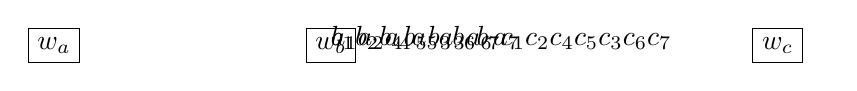
\begin{tikzpicture}[
        nf/.style={text=black!60},
        ne/.style={draw=black!60},
        ts/.style={}]  
        \tikzset{grow'=up}
        \tikzset{sibling distance=0pt}
        \tikzset{level 1/.style={level distance=32pt}}
		\tikzset{level 2/.style={level distance=28pt}}
		\tikzset{level 3+/.style={level distance=26pt}}
			\begin{scope}[xshift=-100pt]
			\Tree 
				[.\node[draw] {$w_a$};
				\edge[draw=none];
					[.{$a_1$}
						[.{$a_2$}
							[.{$a_4$}
								\edge[dotted]; {\hphantom{\dots}}
								\edge[dotted]; {\hphantom{.}}
							]
							[.{$a_5$}
								\edge[dotted]; {\hphantom{.}}
								\edge[dotted]; {\hphantom{\dots}}
							]
						]
						[.{$a_3$}
							[.{$a_6$}
								\edge[dotted]; {\hphantom{\dots}}
								\edge[dotted]; {\hphantom{.}}
							]
							[.{$a_7$}
								\edge[dotted]; {\hphantom{.}}
								\edge[dotted]; {\hphantom{\dots}}
							]
						]
					]
				]
			\end{scope}
			\Tree 
				[.\node[draw] {$w_b$};
				\edge[draw=none];
					[.{$b_1$}
						[.{$b_2$}
							[.{$b_4$}
								\edge[dotted]; {\hphantom{\dots}}
								\edge[dotted]; {\hphantom{.}}
							]
							[.{$b_5$}
								\edge[dotted]; {\hphantom{.}}
								\edge[dotted]; {\hphantom{\dots}}
							]
						]
						[.{$b_3$}
							[.{$b_6$}
								\edge[dotted]; {\hphantom{\dots}}
								\edge[dotted]; {\hphantom{.}}
							]
							[.{$b_7$}
								\edge[dotted]; {\hphantom{.}}
								\edge[dotted]; {\hphantom{\dots}}
							]
						]
					]
				]
			\begin{scope}[xshift=100pt]
			\Tree 
				[.\node[draw] {$w_c$};
				\edge[draw=none];
					[.{$c_1$}
						[.{$c_2$}
							[.{$c_4$}
								\edge[dotted]; {\hphantom{\dots}}
								\edge[dotted]; {\hphantom{.}}
							]
							[.{$c_5$}
								\edge[dotted]; {\hphantom{.}}
								\edge[dotted]; {\hphantom{\dots}}
							]
						]
						[.{$c_3$}
							[.{$c_6$}
								\edge[dotted]; {\hphantom{\dots}}
								\edge[dotted]; {\hphantom{.}}
							]
							[.{$c_7$}
								\edge[dotted]; {\hphantom{.}}
								\edge[dotted]; {\hphantom{\dots}}
							]
						]
					]
				]
			\end{scope}
			\begin{scope}[xshift=170pt]
				\node (dots) at (0,0) {\dots};
			\end{scope}
    \end{tikzpicture}
    \caption{Abstract canvas of a constructive supertagger's I/O structure.}
    \label{figure:canvas}
\end{figure}

\subsubsection{Geometry-Aware Supertagging}
\label{subsubsection:gas}
A suggestive operationalization of this novel approach is described by~\cite{kogkalidis2022geometryaware}; we'll expand upon it here.
First off, the spatiotemporal dependencies we seek to implement do not follow the inductive biases of any run-of-the-mill architecture we may find precompiled in some machine learning library.
The closest paradigm available are graph neural networks (GNNs), which are essentially the most general class of neural architectures, suitable for learning on arbitrary graphs and manifolds (points, sequences, canonical grids, trees -- these are all just very specific instances of graphs: every neural network is a subclass of a graph neural network).
GNNs are usually formulated on the basis of some graph structure, where primitive graph entries (edges, nodes or both) are iteratively updated in a series of so-called \textit{message passing} rounds.
The concrete implementation of the messaging scheme (including what the flow of communication is and how messages are constructed) are up for deliberation.

In our case, it would be straighforward to add direct messaging components that implement exactly the spatiotemporal dependencies described earlier.
But this lacks subtlety, making no attempt at exploiting the regularity of the output space; sure -- it may be neither sequence nor tree, but it's not an ad-hoc graph either!
Computationally, this would not bode very well either; the number of interactions to compute would be upper bound by the series:
\begin{equation}\label{equation:dense_graph}
\sum_{k=0}^{m := \mathrm{max}_i^n ~ \mathrm{depth}(t_i)}
	\Big(
	\hspace{-22.5pt}
	\underbrace{\vphantom{\sum\nolimits_{k'}^{k}} 2^{k}n}_{\text{\# prediction targets}}
	\hspace{-5pt}
	\times
	~~~
	\big(
	\underbrace{\sum\nolimits_{k'=0}^{k-1} 2^{k'}n}_{\text{\# context nodes}}
	~~
	+ 
	\underbrace{\vphantom{\sum\nolimits_{k'}^{k}}  n}_{\text{input length}}
	\hspace{-10pt}
	\big)
	\Big)
%= \frac{2}{3}(4^{d+1} - 1) \cdot n^2
\end{equation}
whose memory footprint grows as $O(2^{2m} n^2)$, scaling quadratically with sequence length and exponentially with twice the maximal tree depth -- yikes.
To keep this beast under check, we would do well to utilize the output's geometric constants, namely the words.
A reasonable way to do that would be as state tracking vectors (fixed both in count and in length).
Akin to RNN hidden states, these shall be iteratively updated by the decoding process, while simultaneously reining it in.
Practically, each decoding step shall be conditioned on the current states, with each state (word) informing only the nodes it is associated with (the supertag it will decode into) in a one-to-many fashion, i.e. $n$ parallel messaging rounds, each from a \textit{single} state to the (maximally) $2^k$ nodes above.
Conversely, after the step has concluded, states will receive feedback from the nodes last predicted, again respecting word boundaries, now in a many-to-one fashion, i.e. again $n$ parallel messaging rounds, now from the $2^k$ freshly decoded states back to the single state they are assocciated with (originate from).
Unlike the naive approach, the setup maintains the word/supertag alignment while also structurally fusing the input- and output-level interactions sources.
Nodes are indirectly informed by all \textit{local} nodes below, with a much more endearing complexity of just:
\begin{equation}
\sum_{k=0}^{m}
	\underbrace{2^{k} n}_{\text{prediction messages}}
	+
	\underbrace{2^{k} n}_{\text{feedback messages}}
\end{equation}
which now grows as $O(2^m n)$.

Of course, something is amiss: the depth-wise intra-tree interactions may well be captured, but the inter-tree ones are unaccounted for.
In the same vein as before, we may bypass this by having the state vectors communicate with one another after each local feedback around, allowing non-local autoregressive context flows.
Having this done globally (all words communicating with all words) is certainly feasible and still preferrable to (\ref{equation:dense_graph}), but suboptimal: it inserts a $mn^2$ memory complexity component ($m$ messaging rounds in the cartesian product of words).
A better alternative can be found in the dusty scriptures of old: sliding windows.
Regulating and thresholding state interactions according to their relative distance reinstates computational well-behavedness%
	\footnote{Maybe there was something to the locality of supertagging after all.},
substituting $n^2$ with $n\kappa$ for window size $\kappa$ (basically linear in sequence length) and setting the final memory footprint of the decoder at $O(2^mn +mn)$.
	
Computational considerations aside, this formulation is also conducive to learning.
Having interactions modulated and bottlenecked by state tracking vectors reduces the number of statistical confounds accessible to the model, acting as an implicit regularizer and enforcing a degree of locality to the (otherwise distributed) neural representations.
It also justifies a heterogeneous formulation, which would have different graph elements inhabit different vector spaces.
State vectors are recurrent across depth and inter-communicating across width, thus meriting from high-dimensional representations; with that in mind, they can initially be supplied by an external high-horsepower encoder, solving the initial interfacing with the input sentence. 
Tree nodes, on the other hand, encode a decision over a very small vocabulary and are use-and-forget, justifying a low-dimensional representation.
Finally, implementing the forward, backward and horizontal message passing rounds as separable, parameter-sharing convolutions repeated both across depth as well as width reduces the model's parameter count and provides the inductive biases needed for strong generalization.

\paragraph{Tree Parallel Decoding}
Summarizing, the decoding algorithm consists of the following steps:
\begin{enumerate}
	\item State vectors are initialized by some external encoder.
	\item An empty fringe consisting of $n$ blank nodes is instantiated, one such per word, rooting the corresponding supertag trees.
	\item Until a fix-point is reached (there is no longer any fringe):
		\begin{enumerate}
			\item States project class weights to their respective fringe nodes in a one-to-many fashion. Depending on the arity of the decoded symbols, a next fringe of unfilled nodes is constructed at the appropriate positions.
			\item Each state vector receives feedback in a many-to-one fashion from the just decoded nodes above (what used to be the fringe), yielding tree-contextual states.
			\item The updated state vectors emit and receive messages within their local neighborhoods in a many-to-many fashion, yielding tree- and sequence- contextual states.
		\end{enumerate}
\end{enumerate}
A single iteration of step (iii) over the abstract canvas of Figure~\ref{figure:canvas} is presented in Figure~\ref{figure:decoding_process}.

\begin{figure}
	\tikzset{w/.style={draw, outer sep=5pt}}
	\tikzset{n/.style={}}
    \tikzset{grow'=up}
    \tikzset{sibling distance=0pt}
    \tikzset{level 1/.style={level distance=32pt}}
	\tikzset{level 2/.style={level distance=28pt}}
	\tikzset{level 3+/.style={level distance=26pt}}
    	t=0\textsuperscript{-}\hfill\begin{subfigure}{0.85\textwidth}
	\begin{tikzpicture}
			\begin{scope}[xshift=-100pt]
			\Tree 
				[.\node[w] {$w_a$} ;
				\edge[draw=none];
					[.{?}
					]
				]
			\end{scope}
			\Tree 
				[.\node[w] {$w_b$};
				\edge[draw=none];
					[.{?}
					]
				]
			\begin{scope}[xshift=100pt]
			\Tree 
				[.\node[w] {$w_c$};
				\edge[draw=none];
					[.{?}
					]
				]
			\end{scope}
			\begin{scope}[xshift=170pt]
				\node (dots) at (0,0) {\dots};
			\end{scope}
    \end{tikzpicture}
    \end{subfigure}\\[\midsep]
    	t=0\textsuperscript{(a)}\hfill\begin{subfigure}{0.85\textwidth}
	\begin{tikzpicture}
			\begin{scope}[xshift=-100pt]
			\Tree 
				[.\node[w] {$w_a$} ;
				\edge[->];
					[.{$a_1$}
						[.{?}
						]
						[.{?}
						]
					]
				]
			\end{scope}
			\Tree 
				[.\node[w] {$w_b$};
				\edge[->];
					[.{$b_1$}
						[.{?}
						]
						[.{?}
						]
					]
				]
			\begin{scope}[xshift=100pt]
			\Tree 
				[.\node[w] {$w_c$};
				\edge[->];
					[.{$c_1$}
						[.{?}
						]
						[.{?}
						]
					]
				]
			\end{scope}
			\begin{scope}[xshift=170pt]
				\node (dots) at (0,0) {\dots};
			\end{scope}
    \end{tikzpicture}
    \end{subfigure}\\[\midsep]
    	t=0\textsuperscript{(b)}\hfill\begin{subfigure}{0.85\textwidth}
	\begin{tikzpicture}
			\begin{scope}[xshift=-100pt]
			\Tree 
				[.\node[w] (wa) {$w_a$} ;
				\edge[<-];
					[.{$a_1$}
						[.{?}
						]
						[.{?}
						]
					]
				]
			\end{scope}
			\Tree 
				[.\node[w] (wb) {$w_b$};
				\edge[<-];
					[.{$b_1$}
						[.{?}
						]
						[.{?}
						]
					]
				]
			\begin{scope}[xshift=100pt]
			\Tree 
				[.\node[w] (wc) {$w_c$};
				\edge[<-];
					[.{$c_1$}
						[.{?}
						]
						[.{?}
						]
					]
				]
			\end{scope}
			\begin{scope}[xshift=170pt]
				\node (dots) at (0,0) {\dots};
			\end{scope}
    \end{tikzpicture}
    \end{subfigure}\\[\midsep]
  	t=0\textsuperscript{(c)}\hfill\begin{subfigure}{0.85\textwidth}
	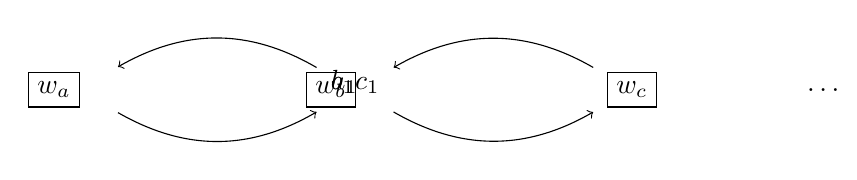
\begin{tikzpicture}
			\begin{scope}[xshift=-100pt]
			\Tree 
				[.\node[w] (wa) {$w_a$} ;
				\edge[draw=none];
					[.{$a_1$}
						[.{?}
						]
						[.{?}
						]
					]
				]
			\end{scope}
			\Tree 
				[.\node[w] (wb) {$w_b$};
				\edge[draw=none];
					[.{$b_1$}
						[.{?}
						]
						[.{?}
						]
					]
				]
			\begin{scope}[xshift=100pt]
			\Tree 
				[.\node[w] (wc) {$w_c$};
				\edge[draw=none];
					[.{$c_1$}
						[.{?}
						]
						[.{?}
						]
					]
				]
			\end{scope}
			\begin{scope}[xshift=170pt]
				\node (dots) at (0,0) {\dots};
			\end{scope}
			\draw[->] (wa) to[bend right] (wb);
			\draw[->] (wb) to[bend right] (wc);
			\draw[<-] (wa) to[bend left] (wb);
			\draw[<-] (wb) to[bend left] (wc);
    \end{tikzpicture}
    \end{subfigure}\\[\midsep]
    	t=1\textsuperscript{(a)}\hspace{18pt}\begin{subfigure}{0.85\textwidth}
	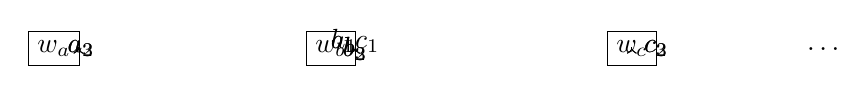
\begin{tikzpicture}
			\begin{scope}[xshift=-100pt]
			\Tree 
				[.\node[w] (wa) {$w_a$} ;
				\edge[draw=none];
					[.{$a_1$}
						[.\node[n] (a2) {$a_2$};
							[.{?}
							]
							[.{?}
							]
						]
						[.\node[n] (a3) {$a_3$};
							[.{?}
							]
							[.{?}
							]
						]
					]
				]
			\end{scope}
			\Tree 
				[.\node[w] (wb) {$w_b$};
				\edge[draw=none];
					[.{$b_1$}
						[.\node[n] (b2) {$b_2$};
							[.{?}
							]
							[.{?}
							]
						]
						[.\node[n] (b3) {$b_3$};
							[.{?}
							]
							[.{?}
							]
						]
					]
				]
			\begin{scope}[xshift=100pt]
			\Tree 
				[.\node[w] (wc) {$w_c$};
				\edge[draw=none];
					[.{$c_1$}
						[.\node[n] (c2) {$c_2$};
							[.{?}
							]
							[.{?}
							]
						]
						[.\node[n] (c3) {$c_3$};
							[.{?}
							]
							[.{?}							]
						]
					]
				]
			\end{scope}
			\begin{scope}[xshift=170pt]
				\node (dots) at (0,0) {\dots};
			\end{scope}
			\draw[->] (wa) to[bend left] (a2);
			\draw[->] (wb) to[bend left] (b2);
			\draw[->] (wc) to[bend left] (c2);
			\draw[->] (wa) to[bend right] (a3);
			\draw[->] (wb) to[bend right] (b3);
			\draw[->] (wc) to[bend right] (c3);
    \end{tikzpicture}
    \end{subfigure}\\[\midsep]
    \caption{The first decoding iteration from start to finish.}
    \label{figure:decoding_process}
\end{figure}


\subsubsection{Implementation}
We are no longer in the distant past; high-level fluff will no longer suffice.
Scientific integrity and lack of peer approval also compel explication.
The paragraphs to follow detail how the abstract pipeline is executed in practice. 
Consider yourself warned: you are urged to skip to the next section if sensitive to machine learning jargon, or the calendar year in your frame of reference is greater or equal to 2026 (I expect every single word to be obsolete by then).

\paragraph{Node Embeddings}
State vectors are temporally dynamic and of size $d_w$; they are initialized to $\mathbf{h}_{0:n}^0 \in \mathbb{R}^{n\times d_w}$ by some external encoder, and are then updated through the fix-point iteration of three message passing rounds, as described in the next paragraphs.
Tree nodes, on the other hand, are not subject to temporal updates, but instead become dynamically ``revealed'' by the decoding process. 
Their representations of size $d_n$ are computed on the basis of (i) their primitive symbol and (ii) their position within a tree.

Primitive symbol embeddings are obtained from a standard embedding table $W_e: \mathcal{S} \to \mathbb{R}^{d_n}$ that contains a distinct vector for each symbol in the set of primitives $\mathcal{S}$. 
When it comes to embedding positions, we are presented with a number of options.
It would be straightforward to fix a vocabulary of positions, and learn a distinct vector for each.
But this is neither inclusive nor elegant: it imposes an ad-hoc bound to the shape and size of tree nodes that can be encoded (contradicting the constructive paradigm), and fails to account for the compositional nature of trees.
The structure-conscious route requires noting that \textit{paths} over binary branching trees form a semi-group, i.e. they consist of two primitives (namely a left and a right path), and an associative non-commutative binary operator that binds two paths together into a single new one.
The archetypical example of a semigroup is matrix multiplication; we therefore instantiate a tensor $P \in \mathbb{R}^{2 \times n_d \times n_d}$ encoding each of the two path primitives as a linear map over symbol embeddings.
From the above we can derive a function $p$ that converts positions to linear maps, by performing consecutive matrix multiplications of the primitive weights, as indexed by the binary word of a node's position; e.g. the linear map corresponding to position $12_{10} = 0011_{2}$ would be $p(12) = P_0P_0P_1P_1 \in \mathbb{R}^{d_n \times d_n}$.
We flatten the final map by evaluating it against an initial seed vector $\rho_0 \in \mathbb{R}^{d_n}$, corresponding to the tree root (or the initial hidden state in the RNN paradigm).
To stabilize training and avoid vanishing or exploding weights and gradients, we model paths as \textit{unitary} transformations by parameterizing the two matrices of $P$ to orthogonality using the exponentiation trick on skew-symmetric bases~\cite{bader2019computing,lezcano2019trivializations}.
Now, let tree node $s_{i, k}$ contain symbol $\sigma \in \mathcal{S}$; its embedding $n_{i,k}$ will be agnostic to its tree index $i$ and given as the element-wise product of its tree-positional and content embeddings:
\begin{equation}
n_{i, k} = p(k)(\rho_0) \odot \left(W_e(\sigma)\right) \in \mathbb{R}^{d_n}
\end{equation}
The embedder is then essentially an instantiation of a unitary RNN~\cite{arjovsky2016unitary}, except applied on tree paths rather than symbol sequences.%
	\footnote{Concurrently, \citet{bernardy2022assessing} follow a similar approach in teaching a unitary RNN to recognize Dyck words, and find the unitary representations learned to respect the compositional properties of the task.
	Here we go the other way around, using the unitary recurrence exactly because we expect them to respect the compositional properties of the task.}
Since paths are shared across trees, their representations are in practice efficiently computed once per batch for each unique tree position during training, and stored as fixed embeddings during inference.

\paragraph{Node Prediction} 
Assuming at step $\tau$ a sequence of globally contextualized states $\mathbf{h}^{\tau}_{0:n}$, we need to use each element $h^{\tau}_i$ to obtain class weights for all of the node neighborhood $\mathcal{N}_{i, \tau}$ consisting of all nodes (if any) of tree $t_i$ that lie at depth $\tau$.%
	\footnote{That's a lot of indexing operations. Look at figure~\ref{figure:canvas} and assume an enumeration that starts from 0 for timesteps and sequence positions and 1 for node positions. Then $\mathcal{N}_{1,2}$ would be $\{b_4, b_5, b_6, b_7 \}$.}
We start by down-projecting the state vector into the node's dimensionality using a linear map $W_n$.
The resulting feature vectors are indistinguishable between all nodes of the same tree -- to tell them apart (and obtain a unique prediction for each), we gate the feature vectors against each node's positional embedding.
From the latter, we obtain class weights by matrix multiplying them against the transpose of the symbol embedding table, as standard practice compels~\cite{press-wolf-2017-using}:
\begin{equation}
\mathrm{weights}_{i,k} = \left(p(k)(\rho_0) \odot W_n h^{\tau}_i\right) W_e^\top
\end{equation}
The above weights are converted into a probability distribution over the alphabet symbols $\mathcal{S}$ by application of the $\mathrm{softmax}$ function. 
%The distribution can be sampled over to generate a concrete prediction.

\paragraph{Autoregressive Feedback}
To update the states for the next iteration, we must first provide autoregressive feedback from the last decoded nodes.
We do so using a heterogeneous message-passing scheme based on graph attention networks~\cite{velivckovic2018graph,brody2021attentive}.
First, we use a a linear map $W_b$ to down-project the state vector into the nodes' dimensionality.
For each position $i$ and corresponding state $h^\tau_i$, we compute a self-loop score:
\begin{equation}
\tilde{\alpha}_{i,\circlearrowleft,\tau} = w_{a} \cdot (W_b(h^\tau_i) \ ||  \ \mathbf{0})
\end{equation}
where $w_a \in \mathbb{R}^{2d_n}$ a dot-product weight and $\mathbf{0}$ a $d_n$-dimensional zero vector.
Then we use the (now decoded) neighborhood $\mathcal{N}_{i, \tau}$ to generate a heterogeneous attention score for each node $s_{i, k} \in \mathcal{N}_{i, \tau}$:
\begin{equation}
\tilde{\alpha}_{i,k,\tau} = w_a \cdot (h^{\tau}_i \ || \ n_{i, k})
\end{equation}
Scores are passed through a leaky rectifier non-linearity before being normalized to attention coefficients $\alpha$.
These are used as weighting factors that scale the self-loop and input messages, the latter upscaled by a linear map $W_m$:
\begin{equation}
	\tilde{h}^\tau_i = \sum_{s_{i, k} \in \mathcal{N}_{i,\tau}} {\alpha}_{i,k,\tau}W_m n_{i,k} + {\alpha}_{i,\circlearrowleft,\tau} h^\tau_i
\end{equation}
This can also be seen as a dynamic residual connection -- $\alpha_{i,\circlearrowleft,\tau}$ acts as a gate that decides how open the state's representation should be to node feedback (or conversely, how strongly it should retain its current values).
States receiving no node feedback (i.e. states that have completed decoding one or more time steps ago) are thus protected from updates, preserving their content.
In practice, attention coefficients and message vectors are computed for multiple attention heads independently as done by~\citet{vaswani2017attention}, but these are omitted from the above equations to avoid cluttering the notation.

\paragraph{Sequential Feedback}
At the end of the node feedback stage, we are left with a sequence of locally contextualized states $\tilde{h}^\tau_i$.
The sequential structure can be seen as a fully connected directed graph, nodes being states (words) and edges tabulated as the square matrix $\mathcal{E}$, with entry $\mathcal{E}_{i, j}$ containing the relative distance between words $i$ and $j$.
%$\mathcal{E}$ labeled by relative distances between word pairs.
We embed these distances into the encoder's vector space using an embedding table $W_r \in \mathbb{R}^{2\kappa \times d_w}$, where $\kappa$ the maximum allowed distance, a hyper-parameter.
Edges escaping the maximum distance threshold are truncated rather than clipped, in order to preserve memory and facilitate training, leading to a natural segmentation of the sentence into (overlapping) chunks.
Following standard practices, we project states into query, key and value vectors~\cite{vaswani2017attention}, and compute the attention scores between words $i$ and $j$ using relative-position weighted attention~\cite{shaw-etal-2018-self}:
\begin{equation}
\tilde{a}_{i,j} = d_w^{-1/2}~(W_q \tilde{h}^\tau_i \odot W_r\mathcal{E}_{i,j}) \cdot W_k\tilde{h}^\tau_j
\end{equation}
From the normalized attention scores we obtain a new set of aggregated messages:
\begin{equation}
m_{i,t}' = \sum_{j \in \{0..s\}} \frac{\mathrm{exp}(\tilde{a}_{i,j}) W_v\tilde{h}^\tau_j}{
\sum_{k\in \{0..s\}}
\mathrm{exp}(\tilde{a}_{i,k})}
\end{equation}
Same as before, queries, keys, values, edge embeddings and attention coefficients are distributed over many heads. 
Aggregated messages are passed through a swish-gated feed-forward layer~\cite{dauphin2017language,shazeer2020glu} to yield the next sequence of state vectors:
\begin{equation}
h^{\tau+1}_i = W_3\left(\mathrm{swish}_1(W_1 m_{i,\tau}')\odot W_2m_{i,\tau}'\right)
\end{equation}
where $W_{1,2}$ are linear maps from the encoder's dimensionality to an intermediate dimensionality, and vice versa for $W_3$.

\paragraph{Putting Things Together}
We compose the previously detailed components into a single layer, which acts as a sequence-wide, recurrent-in-depth decoder.
We insert skip connections between the input and output of the message-passing and feed-forward layers~\cite{he2016deep}, and subsequently normalize each using root mean square normalization~\cite{zhang2019root}.

\subsubsection{Experiments \& Results}
\paragraph{Datasets}
Testing the architecture on multiple datasets is good practice for multiple reasons, the least cynical being that it helps us better affirm its potential.%
	\footnote{The rest I leave open to interpretation.}
Hence, we shall employ it not just on \AE thel but also on the two versions of the CCGbank, as well as the French TLGbank; in total, 4 different datasets spanning three languages and as many grammar formalisms.

\begin{table}
    \centering
    \small{
    \begin{tabular}{@{}l@{\qquad}c@{\quad}c@{\qquad}c@{\qquad}c@{}}
        & \multicolumn{2}{c}{\textbf{\textit{CCGbank}}} 
        & \textbf{\textit{TLGbank}}
        & \textbf{\textit{\AE thel}}\\ 
        & \textit{original} & \textit{rebank} & & ($\mathtt{1.0.0a4}$)\\
        \toprule
        \textbf{Primitives}     & 37        & 40        & 27        & 81\\
        ~ Zeroary           & 35        & 38        & 19        & 31\\ 
        ~ Binary            & 2         & 2         & 8         & 50\\
        \midrule
        \textbf{Categories}     & 1\,323      & 1\,619      & 851      & 5\,762\\
        ~{in train}         & 1\,286      & 1\,575      & 803      & 5\,146\\
        ~{depth avg.}       & 1.94      & 1.96      & 1.99     &   1.82\\
        ~{depth max.}       & 6         & 6         & 7        & 35*\\ 
        \midrule
        \textbf{Test Sentences} & 2\,407      & 2\,407      & 1\,571**    & 5\,770 \\
        ~{length avg.}      & 23.00     & 24.27     & 27.58    &  16.52\\
        \midrule
        \textbf{Test Tokens}    & 55\,371     & 56\,395     & 44\,302     & 95\,331\\
        ~ Frequent {(100+)}   & 54\,825     & 55\,690     & 43\,289     & 91\,503\\
        ~ Uncommon {(10-99)}  & 442       & 563       & 833       & 2\,639\\
        ~ Rare {(1-9)}        & 75        & 107       & 149       & 826\\
        ~ Unseen {(OOV)}      & 22        & 27        & 31        & 363\\
        \addlinespace
        	\multicolumn{5}{@{}l}{*A beautiful conjunction of 35 noun phrases.}\\
      	\multicolumn{5}{@{}l}{**Random but consistent train/dev/test split of 80/10/10.}
    \end{tabular}}
    \caption{Bird's eye view of datasets employed and relevant statistics. Test tokens are binned according to their corresponding categories' occurrence count in the respective dataset's training set. Token counts are measured before pre-processing. Unique primitives and tree depths for the type-logical datasets are counted \textit{after} binarization.}
    \label{table:datasets}
\end{table}


A high-level overview of the datasets is presented in Table~\ref{table:datasets}.
The English CCGbank and its refined version~\cite[rebank]{honnibal2010rebanking} stand out in having combinatory categories as their supertags, built with the aid of two binary slash operators.
Combinatory rules take care of shifting, raising and function composition, allowing the lexicon to remain small and simple.
The key difference between the two versions lies in their tokenization and the plurality of categories assigned, the latter containing more assignments and a more fine-grained set of syntactic primitives, which in turn make it a slightly more challenging evaluation benchmark.
In more familiar grounds we have the French TLGbank, \AE thel's distant but cherished uncle. 
It uses modalities for control purposes, licensing or restricting the applicability of rules related to non-local syntactic phenomena.
Its supertags are therefore multimodal Lambek types, the tree representations of which are not strictly binary; to make compatible with the architecture with minimal effort, we cast unary operators into pseudo-binaries by inserting an artificial terminal tree in a fixed slot within them.
A similar strategy is applied to \AE thel (which I assume is by now familiar).
Unary branches are shortened by first merging diamond-box pairs into a single composite operator, and then iteratively merging adjunct (resp. complement) markers (either plain or composite) with the subsequent (resp. preceding) binary operator.
The new symbols correspond to notational and temporal shorthands for multiple decisions compressed in a single time step, making for an unambiguous and invertible representational translation at the cost of an enlarged primitive alphabet.
These shorthands are not to be confused with the ones we experimented with earlier in Section~\ref{subsection:snmt}.
Back then, we were creating shorthands for frequent (sub-)types (self standing trees), whereas here we are establishing representational shorthands for composite type operators (tree constructors) -- see Figure~\ref{figure:tree_compression} for an example.%
	\footnote{If you're really really observant here, you might see a potential problem with this. 
	If you can't, I'll spoil it for you.
	Some of the composite alphabet symbols may appear in the test set (or in the wild) without having ever appeared in the training set.
	These would be impossible to predict, even in the constructive setting -- not because they're absent from the vocabulary, but because there's no usage examples to learn from!
	In fact, one such symbol exists, corresponding to the type/tree pattern $\dxdia{x}\dxbox{x}\ddia{cmpbody} \textvisiblespace \li \textvisiblespace$ for hypothesizing a deeply nested body of a complementizer -- it has 3 occurrences in the dev set and 1 in the test set.
	This is basically the zipfian tai of the zipfian tail -- we'll let it slide without rearranging the train/dev/test split, as it poses an innocuous and fun little challenge and an easter egg of shorts.
	Obviously, dropping the practical restriction for binarity would solve the problem, at the cost of elongated trees and the loss of architectural uniformity.}

\begin{figure}
		\begin{subfigure}[t]{0.5\textwidth}
		\centering
		\begin{tikzpicture}
		    [t/.style={text height=1.5ex, text depth=.25ex, rectangle, outer sep=0pt,font=\small},
		    node distance=10pt,
		    tree/.style={very thick},
		    link/.style={dashed}]
		\tikzset{idx/.style={dotted, thick}}
        \tikzset{grow'=up}
        \tikzset{sibling distance=0pt}
        \tikzset{level 1/.style={level distance=32pt}}
		\tikzset{level 2/.style={level distance=28pt}}
		\tikzset{level 3+/.style={level distance=26pt}}
		\Tree
		[.${\li}$
			[.$\ddia{whbody}$
				[.$\li$
					[.$\dxdia{x}$
						[.$\dxbox{x}$
							[.$\ddia{mod}$
								[.$\dbox{mod}$
									[.$\li$
										$\infp[s]$
										$\infp[s]$
									]
								]
							]
						]
					]
					$\svi[s]$
				]
			]
			$\whq[s]$
		]
		\end{tikzpicture}
		\caption{Original decomposition.}
		\end{subfigure}%
		\begin{subfigure}[t]{0.5\textwidth}
		\centering
		\begin{tikzpicture}
		    [t/.style={text height=1.5ex, text depth=.25ex, rectangle, outer sep=0pt,font=\small},
		    node distance=10pt,
		    tree/.style={very thick},
		    link/.style={dashed}]
		\tikzset{idx/.style={dotted, thick}}
        \tikzset{grow'=up}
        \tikzset{sibling distance=0pt}
        \tikzset{level 1/.style={level distance=36pt}}
		\tikzset{level 2/.style={level distance=32pt}}
		\tikzset{level 3+/.style={level distance=32pt}}
		\Tree
			[.${\li}\ddia{whbody}$
				[.$\li$
					[.$\dxdia{x}\dxbox{x}\ddia{mod}\dbox{mod}\li$
							$\infp[s]$
							$\infp[s]$
					]
					$\svi[s]$
				]
				$\whq[s]$
			]
		\end{tikzpicture}
		\caption{With notational shorthands.}
		\end{subfigure}
	\caption{Compactifying the horrifying type of Figure~\ref{figure:hard_abstraction}.}
	\label{figure:tree_compression}
\end{figure}
	
\paragraph{Training}
A single hyper-parameter setup is shared among all experiments, obtained after a minimal logarithmic search over sensible initial values.
Specifically, we set the node dimensionality $d_n$ to 128 with 4 heterogeneous attention heads and the state dimensionality $d_w$ to 768 with 8 homogeneous attention heads.
The window size for the state-to-state messaging passing rounds is set to 14 (1 self connection, 6 right neighbours and as many left, 1 direct connection to the sequence summary token).
We train using AdamW~\cite{	loshchilov2018decoupled} and a variable learning rate scaled by a linear warmup and cosine decay schedule over 25 epochs, scaled by 10\% for the encoder.
During training we provide strict teacher forcing and apply feature and edge dropout at 20\% chance.
The loss signal is derived as the label-smoothed negative log-likelihood between the network's prediction and the ground truth label.
Base-sized BERT variants are procured from the transformers library~\cite{wolf2020transformers}: RoBERTa for English~\cite{liu2019roberta}, BERTje for Dutch~\cite{de2019bertje} and CamemBERT for French~\cite{martin2020camembert}, all fine-tuned during training.

\paragraph{Evaluation}
We perform model selection on the basis of validation accuracy, and gather the corresponding test scores according to the frequency bins of Table~\ref{table:datasets}.
Table~\ref{table:comparisons} presents our results compared to relevant published literature.
Evidently, our model surpasses established benchmarks in terms of overall accuracy, matching or surpassing the performance of both traditional supertaggers on common categories and constructive ones on the tail end of the frequency distribution, so there's that.

\begin{table}
    \newcommand{\ave}[2]{\multirow{2}{*}{~~\stat{#1}{#2}}}
	\newcommand{\num}[1]{\multirow{2}{*}{#1}}
	
    \centering
    {\smaller
    \begin{tabularx}{1.00\textwidth}{@{}l@{~}Xc@{}c@{}c@{}c@{}c@{}}
    & & \multicolumn{5}{c}{\textbf{accuracy} {(\%)}} \\
    \cmidrule(lr){3-7}
    & \multicolumn{1}{c}{\textbf{model}} & {overall} & {frequent} & {uncommon} & {rare} & {unseen}\\
    \toprule
    \multicolumn{7}{l}{\textit{\textbf{CCGbank (original)}}} \\
    & \multicolumn{1}{l}{Symbol Sequential LSTM /w n-grams}
    & \num{95.99} & \num{96.40} & \num{65.83} &  \multicolumn{2}{c}{\num{8.65\textsuperscript{!}}} \\
    	& \multicolumn{1}{l}{~\smaller\cite{Liu_Ji_Wu_Lan_2021}}\\
    & \multicolumn{1}{l}{Tree Recursive (Feature Embedding)}
    & \num{96.09} & \num{96.44} & \num{68.10} & \num{\textbf{37.40}} & \num{\textbf{3.03}} \\
	& \multicolumn{1}{l}{~\smaller\cite{prange-etal-2021-supertagging}}\\
    & \multicolumn{1}{l}{Cross-View Training}
    & \num{96.10} & \num{--} & \num{--} & \num{--} & \num{n/a} \\ 
    & \multicolumn{1}{l}{~\smaller\cite{clark-etal-2018-semi}}\\
    & \multicolumn{1}{l}{Attentive Convolutions}
    & \num{\textbf{96.25}} & \num{\textbf{96.64}} & \num{71.04} & \num{n/a} & \num{n/a}\\ 
    & \multicolumn{1}{l}{~\smaller\cite{tian2020supertagging}} \\
    \addlinespace
    & \multicolumn{1}{l}{Geometry-Aware Convolutions}
    & \ave{\textbf{96.29}}{0.04}
    & \ave{\textbf{96.61}}{0.04}
    & \ave{\textbf{72.06}}{0.72}
    & \ave{34.45}{1.58}
    & \ave{\textbf{4.55}}{2.87}\\
    & \multicolumn{1}{l}{~\smaller (this work)}\\
    \addlinespace
    \addlinespace
%    %%%%%%%%%%%%%%%%%%%%%%%%%%%%%%%%%%%%%%%%%%%%%%%%%%%%%%%%%%%%%%%%%%%%%%%%%%%%%%%%%%%%%%%%%%%%%%%%%%%%%%%%%
    \multicolumn{2}{L}{\textit{\textbf{CCGbank (rebank)}}} \\
    & \multicolumn{1}{l}{Symbol Sequential Transformer\textsuperscript{\textdagger}}
    & \num{90.68} & \num{91.10} & \num{63.65} & \num{34.58} & \num{\textbf{7.41}} \\
	& \multicolumn{1}{l}{~\smaller\cite{kogkalidis-etal-2019-constructive}}\\
    & \multicolumn{1}{l}{Tree Recursive (GRU)}
    & \num{94.62} & \num{95.10} & \num{64.24} & \num{25.55} & \num{2.47} \\
	& \multicolumn{1}{l}{~\smaller\cite{prange-etal-2021-supertagging}}\\
    & \multicolumn{1}{l}{Tree Recursive (Feature Embedding)}
    &  \num{94.70} & \num{95.11} & \num{68.86} & \num{\textbf{36.76}} & \num{4.94} \\
	& \multicolumn{1}{l}{~\smaller\cite{prange-etal-2021-supertagging}}\\
    \addlinespace
    & \multicolumn{1}{l}{Geometry-Aware Convolutions}
    & \ave{\textbf{95.07}}{0.04}
    & \ave{\textbf{95.45}}{0.04}
    & \ave{\textbf{71.40}}{1.15}
    & \ave{\textbf{37.19}}{1.81} 
    & \ave{{3.70}}{0.00}\\
    & \multicolumn{1}{l}{~\smaller (this work)}\\
    \addlinespace
    \addlinespace
%    %%%%%%%%%%%%%%%%%%%%%%%%%%%%%%%%%%%%%%%%%%%%%%%%%%%%%%%%%%%%%%%%%%%%%%%%%%%%%%%%%%%%%%%%%%%%%%%%%%%%%%%%%
    \multicolumn{7}{l}{\textit{\textbf{French TLGbank}}} \\
%    % \midrule
    & \multicolumn{1}{l}{ELMo \& LSTM Classification}
    & \num{93.20} & \num{95.10} & \num{75.19} & \num{25.85} & \num{n/a}\\
	& \multicolumn{1}{l}{~\smaller\cite{moot2019}}\\
    \addlinespace
    & \multicolumn{1}{l}{Geometry-Aware Convolutions}
    & \ave{\textbf{95.92}}{0.01}
    & \ave{96.40}{0.01} 
    & \ave{\textbf{81.48}}{0.97}
    & \ave{\textbf{55.37}}{1.00} 
    & \ave{\textbf{7.26}}{2.67} \\ 
    & \multicolumn{1}{l}{~\smaller (this work)}\\
    \addlinespace
    \addlinespace
%    %%%%%%%%%%%%%%%%%%%%%%%%%%%%%%%%%%%%%%%%%%%%%%%%%%%%%%%%%%%%%%%%%%%%%%%%%%%%%%%%%%%%%%%%%%%%%%%%%%%%%%%%%   
    \multicolumn{7}{l}{\textit{\textbf{\AE thel}} ($\mathtt{0.4}$)} \\
%    % \midrule
    & \multicolumn{1}{l}{Symbol Sequential Transformer\textsuperscript{\textborn}}
    & \num{83.67} & \num{84.55} & \num{64.70} & \num{50.58} & \num{\textbf{24.55}} \\
	& \multicolumn{1}{l}{~\smaller\cite{kogkalidis-etal-2020-neural}}\\
	\addlinespace
	\addlinespace
    \multicolumn{7}{l}{\textit{\textbf{\AE thel}} ($\mathtt{1.0.0}$)} \\
    & \multicolumn{1}{l}{Geometry-Aware Convolutions}
    & \ave{\textbf{94.08}}{0.02}
    & \ave{95.16}{0.01} 
    & \ave{\textbf{75.55}}{0.02}
    & \ave{\textbf{58.15}}{0.00} 
    & \ave{\textbf{18.37}}{2.73} \\ 
    & \multicolumn{1}{l}{~\smaller (this work)}\\
    \bottomrule
    \addlinespace
    \multicolumn{7}{l}{\textsuperscript{!}Accuracy over both bins, with a frequency-truncated training set.}\\
    \multicolumn{7}{l}{{\textsuperscript{\textdagger}Numbers from~\citet{prange-etal-2021-supertagging}.}}\\
    \multicolumn{7}{l}{{\textsuperscript{\textborn}Parser-integrated model trained with tree sequences spanning less than 140 nodes in total.}}
    \end{tabularx}}
    \caption{Model performance across datasets and compared to recent studies. Numbers are taken from the papers cited unless otherwise noted. For our model, we report averages and standard deviations over 6 runs. Bold face fonts indicate (within standard deviation of) highest performance.}
    \label{table:comparisons}
\end{table}

To investigate the relative impact of each network component, we conduct an ablation study where message passing components are removed from their network in their entirety.
Removing the state feedback component collapses the network into a token-wise separable recurrence, akin to a graph-featured RNN without a hidden-to-hidden affine map.
Removing the node feedback component turns the network into a Universal Transformer~\cite{dehghani2018universal} composed with a dynamically adaptive classification head.
Removing both is equatable to a 1-to-many contextualized token classification that is structurally unfolded in depth.
Our results, presented in Table~\ref{table:ablations}, verify first a positive contribution from both components, indicating the importance of both information sharing axes.
In three out of the four datasets, the relative gains of incorporating state feedback outweigh those of node feedback, and are most pronounced in the case of \AE thel, likely due to its positionally agnostic types.
With the exception of CCGrebank, relinquishing both kinds of feedback largely underperforms having either one, experimentally affirming their compatibility.

\begin{table}
    \centering
    {\small
    \begin{tabular}{@{}l@{\qquad}ccc@{}}
        &  {node feedback only}  & {state feedback only} & {no feedback} \\
        \toprule
        \textit{\textbf{CCGbank} (original)} & -0.05 & -0.01 & -0.08 \\ 
        \textit{\textbf{CCGbank} (rebank)} & -0.12 & -0.04 & -0.07 \\
        \textit{\textbf{French TLGbank}} & -0.13 & -0.14 & -0.23 \\
        \textit{\textbf{\AE thel}} ($\mathtt{1.0.0}$) & -0.24 & -0.12 & -0.39
    \end{tabular}}
    \caption{Absolute difference in overall accuracy when removing the state and node feedback components (averages of 3 repetitions).}
    \label{table:ablations}
\end{table}


\subsubsection{Insights \& Observations}
\paragraph{Advantages}
Obtaining state of the art performance while still being able to predict rare and unseen types with relative reliability is a definite advantage.
Like before, the approach provisions contextual and self-standing representations for atomic components virtually for free.
Unlike before, the architecture boasts an extremely fast inference speed that goes toe-to-toe with conventional discriminative architectures, owing to its temporal upper bound scaling with maximal tree depth (practically a constant, except for really perverse cases).
Structure manipulation is kept to the bare minimum, even in the absence of oracle guidance, maximizing GPU utilization and data parallelism with high efficiency sparse routines~\cite{fey2019fast}.
Operations are batched and temporally iterated across all nodes and sequences without any CPU interruptions.
Each next fringe is dynamically generated on a purely numerical basis.%
	\footnote{By selecting decoded symbols that correspond to tree forming operators, isolating their indices, multiplying them by two (to create left children), offsetting by one (to create right children), and finally interleaving the two to yield both descendants.
In the same vein, the indices of the aligned states are simply the repetition of their respective ancestors' indices.}
The architecture's memory footprint and parameter count are also the product of careful design and thus well under check, facilitating training and parser integration (as we will soon see).
The model takes approximately 5 hours to train on each dataset, and boasts a constant processing speed of 6\,000 \sfrac{tokens}{sec} on a consumer-grade laptop GPU. By comparison, the sequential model takes about 100 hours to converge, and processes about 700 \sfrac{tokens}{sec}, scaling inversely with sentence length.

\paragraph{Supertagging and Sparsity}
Practice aside, the results obtained pose concrete evidence that lexical sparsity, historically deemed the categorial grammar's curse, might well just require a change of perspective to tame and deploy as the answer to the very problem it poses.
Crucially, the architecture's relative gains scale with respect to the task's complexity.
In the original version of the CCGbank, the model is only slightly superior to the next best performing model -- an ad-hoc graph neural network with built in lexical biases (quite literally the ideological antipode of our endeavour).
The difference becomes an order of magnitude wider for the slightly more challenging rebank version.
The effect is maximally pronounced for the harder type-logical datasets.
For the French TLGbank, performance jumps up to CCGbank scales (despite it being significantly smaller and sparser).
For \AE thel, the absolute performance leap is about 10\% compared to the vanilla constructive tagger.
Even though there's some data distance between the two experiments (version gap, different data filtering, etc.) making strict numeric comparisons moot, the sizeable improvement is beyond doubt.
This is clearly to be attributed to increased returns from the rare and uncommon bins.
There is a synergistic effect between the larger population of these bins pronouncing even minor improvements, while at the same time the acquisition of rare categories apparently benefits from their plurality.
Put simply, learning sparse assignments is \textit{easier} in grammars that contain many and diverse rare assignments, and improvements there \textit{matter} more -- especially so if these don't come at the cost of stability at the higher frequency spectrum.
The impact of this finding alone is bigger than the menial architecture itself -- it is basically an open invitation to more elaborate, more strict and more regular lexicalized theories, and a promise that no matter how statistically unruly they might seem, there will always be an architectural solution to accommodate them.
In today's machine learning frenzy, it is a statement of purpose lost: tools for the task, and not tasks for the tools.

\paragraph{Downsides}
Despite its objective success, the methodology is not without limitations.
Most importantly, the parallel nature of the decoder trades inference speed for an incompatibility with greedy algorithms like beam search and an inability to produce local assignment rankings.
Put plainly, obtaining more than the "best" category assignment per word is not straightforward, a fact which can prove harmful for coverage of a downstream parser.
A possible solution would involve branching across multiple tree-slices (i.e. sequences of partial assignments) rather than single predictions, but efficiently computing scores and comparing between complex structures is uncharted territory and not trivial to implement.
The issue is of course not unique to this system, but common to all decoders that perform multiple assignments concurrently -- as such, there is some hope that insights might percolate from one field to another and eventually make their way to us.

\section{Neural Proof Search}
\label{section:npn}
We have made significant progress with supertagging, first removing the scary-looking roadblock of lexical type sparsity, and then producing numbers bigger than any numbers seen before%
	\footnote{Actually, \citet{tian2020supertagging} were reporting even bigger numbers for a while, but it later turned out that these numbers were in error and their real numbers were a lot smaller than the numbers they originally reported.
	An honest mistake, no doubt due to churning out the same architecture 5 times over the span of a year -- they thought you're not supposed to measure performance on rare assignments at all.
	Long story short, don't trust the numbers.}%
, earning a spot at at the top 10 pop hits leaderboard for the next couple of months.
But supertagging alone is not going to take us to the end of the road.
Far from it, in fact, since our chosen logic is extremely permissive, burning away any hope of making do using just the proof-theoretic tools we have available.
The problem is simple: our type assignments, even when fully correct, still allow more proofs than desired -- we need yet another statistical learner on which to outsource the duty of finding which one of these many proofs is the linguistically sensible one.
And once more, the discriminator approach is not going to work: enumerating and ranking all well-formed proofs is a no-go -- we have to build the correct proof from scratch instead.

To move forward we need to look back.
Almost an entire book ago, we had a brief encounter with proof nets, and we saw them at work in the context of $\ILL_{\li}$ (by now rebranded as \NLP).
Back then, we were quick to dismiss them after a moment of shallow appreciation, seeing as they were too complicated of a proof format for conducting search on, and too underspecific of a representational format for showing around.
Lots have changed since, and not for the better; we added modalities, which impose further structure on their own, invisible to proof nets (at least in their unaltered form).
Why then should we turn our attention back to them now?

The blast from the past is justified by the inadequacy of alternatives.
The natural deduction presentation we have predominantly employed is hierarchical and tree-like; assuming perfect processing and regardless of search direction (bottom-up or top-down), computation is temporally bound by the proof depth -- bottlenecked by decisions due, or anticipating decisions to be.
The same is true for most proof-theoretic alternatives (tableaus, the sequent calculus, $\lambda$ terms, etc.).
Decisions cannot be detached from the structure they bind to and help form -- to make a choice requires knowing your options, which in turn requires that previous choices were not just abstractly \textit{made} but concretely \textit{evaluated}.
At the same time, even if the proof is to be dynamically constructed, thus abolishing the need for enumerating all options globally, each local junction point still needs to be exhaustively expanded for the construction to proceed.
Explicit symbolic manipulation and neural representations are inseparably bound, and even though the former can be somewhat localized, it can never be foregone fully.
Practically speaking, type safety is not for free: it costs back-and-forth between the logical and numerical back ends, inhibiting integration.
Proof nets, on the other hand, are the embodiment of data parallelism, the most saught after property of neural computation and the holy grail of efficient training and optimization.
Decision making and validity testing are detached: we must first make all the decisions that are to be made, and only then can we check whether they are structurally legitimate.
This laxness was the very reason we abandoned proof nets in the first place, but it is exactly what makes them so very appealing now.

%What follows is a retrospective revision and expansion of the ideas and experiments of \citet{kogkalidis-etal-2020-neural}.

\subsection{Parsing as Permutation}
So what exactly is the structure of decisions encoded in a proof net?
Recalling our earlier discussion, a proof net is essentially two things and a promise.
First, a sequence of decomposition trees, called a proof frame.
Second, a bijection between atomic formulas of opposite polarities, called axiom links.
The two together make a proof structure -- if it so happens that we can traverse the structure, the promise is kept: it is also a proof net.
The proof frame is deterministically obtained from a sequence of type assignments, and thus irrelevant to this discussion -- in principle, we can assume it to be given from the supertagging component.
The promise of traversability corresponds to the deferred (and also deterministic) validity checking -- it can only be done \textit{given} a proof structure.
The only thing we really have any say on is the axiom links.
Our goal is therefore to design a neural model capable of manipulating sets and building bijections between them -- and not just \textit{any} bijections, but rather only those that are theoretically permitted (traversable, i.e. valid proofs) and linguistically sensible (i.e. not just valid proofs, but also valid parses).

A feeling of apprehension wouldn't be unreasonable at this point; neural models are notoriously ill-fit for discrete and combinatorial optimization.
Pulling us out of this momentary lapse is the folkloric knowledge that a bijection between two ordered sets, or \textit{chains}, can be uniquely represented as a \textit{permutation matrix} -- a boolean valued, doubly stochastic and square matrix that, left-applied to set\textsubscript{1} (in column form), \textit{transports} each of its elements to its pair in set\textsubscript{2}.
Note that the order does not need to be due to some intrinsic property of the set and its elements, but may well be externally imposed -- this is just simply a representational trick.
Considering also that a link is only possible between different instances of the \textit{same} atomic type, the problem naturally reduces to finding not a single, big matrix, but many smaller, independent ones.

This might all be easier to digest with a visual example.
Let's turn our attention to Figure~\ref{figure:rare_teken}, which displays an annotated proof net for the wh-question \texttr{Wat is die rare tekening?}{What is this scary picture?}, with derivation:
\begin{equation}
	\w{wat}~\ddiaintro{whbody}(\lam \Var{0}.\w{is}~\Var{0}~\ddiaintro{su}(\dboxelim{det}\w{die}~(\dboxelim{mod}\w{rare}~\w{tekening})))
\end{equation}
Formula decompositions should be easy to decipher.
Following the polarization induction, we end up with polarity information for all formula nodes, all the way up to leaves -- the only addition to the modus operandi of  Section~\ref{subsection:proofnets} are the unary modal branches, which are polarity preserving.
To be able to tell distinct occurrences of the same atom apart, we associate a unique index to each leaf; the convention followed is irrelevant, but we may as well assume a depth-first left-first sequence-wide enumeration.
We can then use these to refer back to the occurrences of atomic formulas they identify within the proof frame.
Gathering positive and negative leaves, we end up with two ordered sets $P$ and $N$; in this case $P := \{ 0, 2, 5, 7, 9, 10\}$ and $N := \{ 1,3,4,6,8,11\}$.
Each set can then be partitioned according to its elements' types, yielding as many positive as negative subsets, aligned in equinumerous pairs; i our case, positive subsets $P_{\vnw[s]} = \{ 0 \}$, $P_{\svi[s]} = \{5 \}$, $P_{\whq[s]} = \{2\}$, $P_{\np[s]} = \{ 7 \}$  and $P_{\n[s]} = \{ 9, 10 \}$, and their negative counterparts $N_{\vnw[s]} = \{3\}$, $N_{\svi[s]} =\{1 \}$, $N_{\whq[s]} = \{ 11 \}$, $N_{\np[s]} = \{4\}$  and $N_{\n[s]} = \{ 6, 8\}$.
Now, rather than look for the correct bijection between $P$ and $N$, we should be looking for the correct bijections between sets of the same ``type'' and opposite polarity.
All sets except those indexed by $\n[s]$ are singletons, their pairs having but one bijection.
Each of $P_{\n[s]}$ and $N_{\n[s]}$ contains two elements, giving rise to two possible bijections -- a one-in-two choice that captures the entire proof!
The bijection we are in search for is $\pi_{\n[s]} : P_{\n[s]} \biject N_{\n[s]}$, $\pi_{\n[s]}(9)=6$, $\pi_{\n[s]}(10)=8$, which can be represented as the permutation matrix:
\begin{equation}
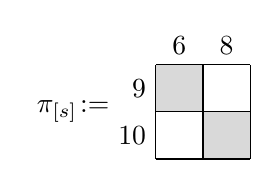
\begin{tikzpicture}[scale=.6]
    \fill[gray!30] (0,1) rectangle +(1,1);
    \node [above] at (0.5, 1) {\checkmark};
    \fill[gray!30] (1,0) rectangle +(1,1);
    \node [above] at (1.5, 0) {\checkmark};
    \node [above] at (0.5,2) {6};
    \node [above] at (1.5,2) {8};
    \node [left] at (0,1.5) {9};
    \node [left] at (0,0.5) {10};
    \node at (-1.75,1) {${\pi}_{\n[s]}\!:=$};
    \draw (0,0) grid (2,2);
\end{tikzpicture}
\end{equation}
Without loss of generality, creating such matrices is what the proof search we need to conduct boils down to -- even if usually we'll have more choices spread among more types.
Needless to say, this is a simplification; structural constraints are only partially imported, in the sense that traversability and well-formedness are not respected by default.
It is not an unreasonable one though; the format is compact, and imports at least some of the structural constraints, faithfully mirroring the definition of a proof structure at least.
Besides, matrices are the bread and butter of machine learning -- we're on the right track.

\begin{figure}
    \resizebox{1\textwidth}{!}{
		\begin{tikzpicture}
		    [t/.style={text height=1.5ex, text depth=.25ex, rectangle, outer sep=0pt,font=\small},
		    node distance=10pt,
		    tree/.style={very thick},
		    link/.style={dashed}]
		\tikzset{frontier/.style={distance from root=200pt}}
		\tikzset{idx/.style={dotted, thick}}
        \tikzset{grow'=up}
        \tikzset{sibling distance=0pt}
        \tikzset{level 1/.style={level distance=36pt}}
		\tikzset{level 2/.style={level distance=32pt}}
		\tikzset{level 3+/.style={level distance=32pt}}
		\Tree
			[.{\w{Wat}} \edge[draw=none];
				[.{$\li$}
					[.{$\ddia{whbody}$}
						[.{$\li$} \edge[dashed] node[left] {$\Var{0}$};
							[.{$\ddia{predc}$}
								[.{$\vnw^+$} \edge[idx, gray!40];
									\node[t] (0) {0};
								]
							]
							[.{$\svi^-$} \edge[idx, gray!40];
								\node[t] (1) {1};
							]
						]
					]
					[.{$\whq^+$} \edge[idx, gray!40];
						\node[t] (2) {2};
					]
				]	
			]		
		\begin{scope}[xshift=75pt]
			\Tree
				[.{\w{is}} \edge[draw=none];
					[.{$\li$}
						[.{$\ddia{predc}$}
							[.{$\vnw^-$} \edge[idx, gray!40];
								\node[t] (3) {3};
							]
						]
						[.{$\li$}
							[.{$\ddia{su}$}
								[.{$\np^-$} \edge[idx, gray!40];
									\node[t] (4) {4};
								]
							] 
							[.{$\svi^+$} \edge[idx, gray!40];
								\node[t] (5) {5};
							]
						]
					]
				]
		\end{scope}
		\begin{scope}[xshift=150pt]
			\Tree
				[.{\w{die}} \edge[draw=none];
					[.{$\dbox{det}$}
						[.{$\li$}
							[.$\n^-$ \edge[idx, gray!40];
								\node[t] (6) {6};
							]
							[.{$\np^+$} \edge[idx, gray!40];
								\node[t] (7) {7};
							]
						]
					]
				]
		\end{scope}
		\begin{scope}[xshift=200pt]
			\Tree
				[.{\w{rare}} \edge[draw=none];
					[.{$\dbox{mod}$}
						[.${\li}$
							[.{$\n^-$} \edge[idx, gray!40];
								\node[t] (8) {8};
							]
							[.{$\n^+$} \edge[idx, gray!40];
								\node[t] (9) {9};
							]
						]
					]
				]
		\end{scope}
		\begin{scope}[xshift=250pt]
			\Tree
				[.{\w{tekening}} \edge[draw=none];
					[.{$\n^{+}$} \edge[idx, gray!40];
						\node[t] (10) {10};
					]
				]
		\end{scope}
		\begin{scope}[xshift=300pt]
			\Tree
				[.{} \edge[draw=none];
					[.{$\whq^{-}$}	\edge[idx, gray!40];
						\node[t] (11) {11};
					]
				]
		\end{scope}
        \draw[<-, idx] (0) -- ($(0) + (0, 2)$) -| (3);
        \draw[->, idx] (8) -- ($(8) + (0, 1)$) -| (10);
        \draw[->, idx] (4) -- ($(4) + (0, 1)$) -| (7);
        \draw[->, idx] (1) -- ($(1) + (0, 1.5)$) -| (5);
        \draw[->, idx] (6) -- ($(6) + (0, 0.55)$) -| (9);
        \draw[->, idx] (11) -- ($(11) + (0, 2.5)$) -| (2);
	    \end{tikzpicture}
    }
    \caption{The two layers of an $\NLPplus$ proof net: a proof frame (below) with its axiom links (above).}
    \label{figure:rare_teken}
\end{figure}

\subsection{Neural Proof Nets}
Permutation matrices may well be matrices, but they're still discrete -- not something we could ever hope to differentiably produce.
In our neural reimaging of axiom links, we need to go for the next best thing: their continuous relaxations.
A soft version of a permutation matrix can be approximated with arbitrary precision by virtue of the Sinkhorn operator~\cite{sinkhorn1964relationship}.
The operator and its underlying theorem state that the iterative normalization (alternating between rows and columns) of a square matrix with positive entries yields, in the limit, a doubly-stochastic matrix, the entries of which are \textit{almost} binary.
Almost binary is binary enough -- we will do just fine without going to the limit.
The positive entry constraint is a minor hickup though.
To bypass it, we can move computation to the logarithmic domain, employing the $\mathrm{log}$-$\mathrm{sum}$-$\mathrm{exp}$ trick in place of standard normalization, which also helps ensure numerical stability.
In that setting, the Sinkhorn normalization of a real-valued square matrix $\mathbf{X}$ is defined as:
\begin{equation}
\mathrm{Sinkhorn}(\mathbf{X})= \lim_{\tau \to \infty}\mathrm{exp}\left(\mathrm{Sinkhorn}^{(\tau)}(\mathbf{X})\right)
\end{equation}
where the induction is given by:
\begin{align}
    \mathrm{Sinkhorn}^{(0)}(\mathbf{X}) &= \mathbf{X} \\
    \mathrm{Sinkhorn}^{(\tau)}(\mathbf{X}) &= \mathcal{T}_r\left(\mathcal{T}_r\left(\mathrm{Sinkhorn}^{(\tau-1)}(\mathbf{X})\right)^\top\right)
\end{align}
and $\mathcal{T}_r$ the row normalization in the log-space:
\begin{equation}
{\mathcal{T}_r(\mathbf{X})}_{i, j} = \mathbf{X}_{i, j} - \mathrm{log}\sum\limits_{r=0}^{N-1}{\mathrm{exp}{(\mathbf{X}_{r, j} - \mathrm{max}(\mathbf{X}_{r, :}))}}
\end{equation}

Used this way, the Sinkhorn operator gives rise to a non-linear activation function that applies on matrices and pushes them towards binarity and bistochasticity, analogous to a 2-dimensional softmax that preserves assignment~\cite{mena2018learning}.
This exotic activation function is the key to efficiently navigating the combinatorially prohibitive landscape of axiom links.%
	\footnote{Recall that the number of possible bijections scales factorially with the cardinality of the sets.}
Where previously we would need to either (i) thoroughly construct and rank all combinations, or (ii) iteratively decode through each element of set\textsubscript{1} while dynamically adjusting set\textsubscript{2} as candidates get excluded, we are now presented with a much more appealing alternative; a temporally bound, backtrack-free operation that translates the structural constraint of bijectivity into highly optimized and fully parallelizable linear algebraic routines.

To apply in the setup envisaged here, all we need to do is assemble matrices containing unnormalized similarity scores in the cartesian product of positive $P_{\chi}$ and negative $N_{\chi}$ occurrences of formula tree leaves, one such matrix $S_{\chi}$ per unique atomic proposition $\chi$ present in a frame; a similar position is advocated by~\citet{moot2008graph}.
Normalizing these scores with Sinkhorn and contrasting the result with the target output (the discrete ground truth permutation $\pi_{\chi}$) amounts to teaching a network an implicit ranking of the set of bijections between the two sets, on the basis of their elements' representations.
If training goes according to plan, the $\pi_{\chi}$-image (resp. $\pi_{\chi}^{-1}$) of each element of $P_{\chi}$ (resp. $N_{\chi}$) will outrank all competing items in $N_{\chi}$ (resp. $P_{\chi}$), i.e. be the largest entry of its row (resp. column) in $S_{\chi}$.
For this to have any chance of success, the mechanism producing $S_{\chi}$, and by extension the representations of $P_{\chi}$ and $N_{\chi}$, will need to be highly contextual.
Embedding a leaf's type, polarity and/or tree position won't cut it -- sequential context is crucial to disambiguate between leaves living in distinct instances of identical types, whereas lexical association context should prove beneficial in resolving derivational ambiguities (rare as they might be).
Coincidentally and to our great fortune, the two constructive supertaggers we have described and implemented in the previous section do in fact provide contextual representations, at exactly this granularity scale -- imagine that!
Happy coincidence aside, the operationalization described is plug-and-play for any supertagger, constructive or otherwise -- the picky requirements on subtype representations can always be satisfied by some third party encoder.
Employing such an encoder might even be for the best, in terms of performance alone -- but for the sake of parameter compression and model reuse, we are given the chance to have the decoding architectures described earlier do double duty as ``proof frame encoders''.
To that end, we simply need to jointly train supertagging and axiom linking in a unified, end-to-end architecture, simultaneously optimizing both objectives.%
	\footnote{
	Another way to see this is as a flipped version of the \textit{linear assignment problem}, where given matrices of representations $P$, $N$, a similarity metric $w$ and target output $\pi$, we wish to learn set element representations and the parameters of a similarity metric $w$ (if any), such that the quantity:
	\[
		\sum_{i, j} \pi_{i,j} \odot \mathrm{Sinkhorn}^{\tau}(S)_{i,j}
	\]
	is maximized, where $S_{i,j} = w(P_i, N_j)$.
}

\subsubsection{Implementation(s)}
Since the original publication of \citet{kogkalidis-etal-2020-neural}, the architecture was revised with minor micro-adjustments, and retrained with each new major adaptation of \AE thel, charting a multidimensional course of only partially compatible successive stops.
Rather than suffocate us all with irrelevant distractions and boring tables of deltas, I think it's best if I stick to describing in detail only the current and most recent implementation, drawing parallels with isolated historical insights only when relevant.

\paragraph{Supertagger Integration}
The architecture combines just as easily with both the symbol sequential and the geometrically informed decoder, requiring only an adaptation of how leaf nodes are indexed and gathered.
Freely reusable as they might be, the contextual representations of either decoder are imperfect: each token can only be informed by tokens that temporally preceded it.
In theory, this means that disambiguation between competing link candidates is back-loaded -- the weight of flipping the scales is on the tokens last decoded. 
It also means that the geometry-aware model is at a disadvanage, since it performs multiple assignments in parallel.
In practice, this is not a major concern -- both integrations perform exceptionally well and quickly fit the training set, making the addition of any extra parameters redundant and a potential threat to generalization; we can stick to using the decoder's representations as is.

Choosing between the two decoders seems like a no brainer at first -- the geometry-aware formulation is significantly faster and more accurate, let alone easier to train (despite these factors usually being in conflict).
But in transitioning to it, we fortfeit the right to algorithmically \textit{search} in the output space.
In practical terms, while we may keep demanding a new proof frame from the symbol sequential supertagger ad infinitum (or until satisfied), the geometric one won't be at all receptive to our pleas -- its greedily decoded proof frame is our one and only chance at a parse.
This limitation becomes especially relevant considering the impenetrable barrier placed by the count invariance property, requiring an equal count of positive and negatlives for every atomic type present (no square matrix otherwise!).
A proof frame that fails to satisfy that property is no good for proof search.
This obstacle can be repurposed to a tool, as long as search is an option -- hard-wiring the constraint into beam search yields a correct-by-construction (yet painfully slow) decoding algorithm, massively increasing computational load but practically ensuring parsability.%
	\footnote{
	Beam searching over the symbol sequential decoder with a beam width $\beta$ means obtaining $\beta$ unique sequences satisfying:
	\[
		\mathrm{argmax}_{\beta}\left(
		\prod_i^n \prod_j^{|| t_i ||} 
		p(s_{\beta, i, j} \ | \ 
			s_{\beta, k, :} : k < i,
			s_{\beta, i, k} : k < j,
			\wseq)
		\right)
	\]
	We can import the count invariance condition by overwriting the probability score $p(s_{\beta, n, ||t_n||} | \dots )$ assigned by the decoder with $-\infty$ when $\mathbf{t}_{0:n}$ fails the check, essentially discarding the sequence and forcing a backtrack.
}
Sticking with the parallel decoder means having to wave such niceties goodbye, at least until some search algorithm is formulated and implemented.
Despite the fact, the drastically improved accuracy and speed translate to a multiplicative increase in the performance-to-compute ratio -- the greedy output of the novel supertagger is practically as good as -- and incomparably faster than -- a vanilla beam search on the original one, but with no guarantee of structural correctness.
Long story short, the geometry-aware decoder is not a no brainer, but it's still the superior choice.

Since the permutations require access to the atoms of goal (succedent) formula, we train the supertagger to produce one, using the input sequence's sentential summary token (the \texttt{[CLS]} token, in jargon) as the stateful decoding seed.
\AE thel's proofs are actually restricted to atomic goal types, allowing us to derive them ``by hand'' by simply counting which of the atomic types has a positive atom too much -- but that offers no vectorial representation we can use.

\paragraph{Neural Permutation Module}
The permutation component may modulate the linking process by providing a parametric and trainable similarity metric.
The current version utilizes a weight vector $w \in \mathbb{R}^{d_n}$ to compute similarity scores between positive and negative vectors as their $w$-weighted inner product.
This is an efficient way to selectively allocate signed weights on the decoder's representations, allowing certain pairwise interactions more prominence than others (or even imposing sparsity to disentangle the two problems, if $L_1$ regularization is employed).
Let's take a second to restate this: the transition from supertagging to full-blown parsing incurs a cost of 128 extra parameters; a relative increase of a paltry 0.0001\%.
What we have in our hands is quite literally the world's \textit{leanest} parser.

\paragraph{Neurosymbolic Integration}
Symbolic processing is handled by the tiny type system that \AE thel rests on, now extended with conversion routines that allow casting proofs to proof nets and back (more in a bit).
The conversion routines allow us to conduct neural proof search in the favorable regime of proof nets, and convert the result to natural deduction format only at the very end, for the sake of sanity testing.
Crucially, the type-checker, originally designed to assert the dataset's type safety, is now repurposed to a tool for verifying the correctness of analyses constructed -- a proof structure that does not constitute a proof net will fail the traversal, throwing an error and alerting us to the fact.
In other words, we can blindly trust anything the parser gives us as correct, at least in the sense of syntactic validity.

\subsubsection{Experiments \& Results}
\paragraph{Training}
The unified architecture is end-to-end differentiable, and can be jointly trained on both the supertagging and the axiom linking tasks simultaneously.
The supertagging objective remains exactly as before, whereas the linking loss is obtained as the negative log likelihood between the Sinkhorn-normalized activations and the discrete ground truth labels (identical to standard multiclass classification).
Given that proof frames are a priori known in training and considering that teacher forcing ensures the correct autoregressive interactions, we may simply proceed with isolating the leaves out of the decoder's representations.
Leaf representations are binned according to their sentential index, atomic type and polarity (e.g. a single bin would be all occurrences of a positive $\np[s]$ in sentence \#13 of the input batch).
Each bin is zipped with its opposite polarity counterpart, and their element-wise similarity scores are computed via the chosen metric.%
	\footnote{Note that the zipping function is not \textit{the} similarity metric but the pairwise application of one. 
	In other words, the agreement scores are independently computed between pairs of elements from the two sets.
	This is necessary to account for the variably sized sets encountered without ad-hoc padding, but also to ensure that the end operator is permutation invariant.}
Similarity scores are normalized by a fixed number of Sinkhorn iterations -- three iterations suffice to produce sharp activations without eroding the gradient updates.
Similarity scores and Sinkhorn normalizations are computed in parallel and batched across bins of the same size (i.e. according to the bijected sets' cardinality) -- a faster alternative would be to pad them to a fixed size using some arbitrarily low constant as a padding value, but the difference is minor and not worth the memory overhead. 

The joint architecture takes longer to train than the stand-alone tagger, owing to the slower forward and backward passes, but also due to the increased number of epochs required to reach convergence.
The linking task is surprisingly fast to converge, but its inclusion is detrimental to supertagging, as its loss term dominates the sum early on.
Since accurate supertagging is a prerequisite to parsing, linking loss is scaled by 10\% to promote smoother training curves and a healthier task balance.
To nudge the model away from local optima induced by gradient conflict, one of the two losses is occassionally zeroed out with a 20\% chance.

\paragraph{Evaluation}
During evaluation and inference, the decoder has to rely on its own output, as the ground truth frame is unknown.
When decoding completes, the output must first be ``parsed'' into types proper.
Assuming no structural integrity issues, leaf positions are indexed, keeping track of their polarities and atomic types -- the result is a proof frame.
For the frame to be an eligible starting point for proof search, it must satisfy the count invariance property, which is dynamically asserted on the spot.
If it does, leaf representations are extracted and binned and their agreement scores are computed and normalized like before (except sequentially for each sentence).
In the event that the local discretization (i.e. rounding) of a normalized matrix does not correspond to a bijection, we resort to an explicit combinatorial optimization via the Hungarian method, using the normalized scores as assignment weights.
In either case, the pairings obtained correspond to axiom links, which are traversed to produce a proof (more on that in a bit).

We proceed with evaluation with no training wheels: no pre- or post- processing, no tokenization or chunking oracles, and no length, depth or
frequency thresholding. All scores reported are the average of three repetitions.
Numeric evaluation requires a way to compare proofs.
The first and most transparent thing to consider are sentential- (or proof-) level performance metrics, where there's two axes of interest; axis one is whether we could have gotten or did get a proof, and axis two is whether that proof could be or was the correct one.
The key results are presented in Table~\ref{table:key_results}.

\begin{table}[h]
	\centering
	\begin{tabular}{@{}c@{\qquad}c@{}}
		\textbf{parsability}	&
		\textbf{coverage} \\
		\smaller(some proof obtainable) &
		\smaller(some proof obtained) \\
		\toprule
		\stat{87.35}{0.18} &
		\stat{85.56}{0.22} \\
		\addlinespace
		\textbf{frame accuracy} &
		\textbf{accuracy}\\
		\smaller(correct proof obtainable) & 
		\smaller(correct proof obtained)\\
		\toprule
		\stat{57.76}{0.55} & 
		\stat{55.63}{0.55}\\
	\end{tabular}
	\caption{Sentential-level evaluation of the parser.}
	\label{table:key_results}	
\end{table}

On the bottom right, accuracy corresponds to the proportion of sentences assigned a proof that satisfies \textit{strict syntactic equality} to the ground truth one, and stands at a 55.63\%.
The significance of this number is easy to miss, considering the unforgiving rigidness of the metric and the demanding nature of the task -- proof equality means having \textit{perfectly} captured the input's function-argument structures, functional types and dependency roles.
By comparison, the state of the art in CCGbank parsing is currently 54\%~\cite{DBLP:journals/corr/abs-2109-10044} -- which is only to say that the two tasks, despite their obvious differences, are now very proximal in performance, despite type-logical grammars being traditionally dismissed as ``too complex''.
Less promising is the average coverage, i.e. the proportion of sentences assigned any proof at all, lying at a modest 85.56\%.
To find the culprit for this lacking result, we measure parsability, i.e. the proportion of analyses whose proof frame satisfies the count invariance property.
Evidently, only 87.35\% of the input is amenable to proof search at all.
Despite appearances, this is actually quite reasonable considering the severe architectural limitation of being confined to the one single best proof frame.
It also goes to show that the permutation strategy is incredibly robust; 97.95\% of the parsable sentences are \textit{actually} parsed, with the remaining 2.05\% of the errors being due to a structural link error (i.e. a proof structure that cannot be traversed).
To put this in context, only 2\% of the parsable sentences contain \textit{any} structural error among \textit{any} of their permutation bijections among \textit{any} of the atomic types present.
In other words, the traversability condition that makes a proof structure a proof net has been almost perfectly captured, despite remaining implicit throughout the training process, both in terms of representations used and of the loss signal backpropagated.
More than just incredibly robust, the permutations are extremely accurate.
This is made evident when considering the proportion of correct proofs to correct frames, which lies at an astonishing 96.31\%.
Put plainly, the number suggests that an error-free proof is \textit{practically guaranteed} from an error-free frame.
The results as a whole paint a clear picture that takes little effort to interpret: the performance bottleneck is on the supertagging module rather than the permutation module.

\begin{table}
	\centering
	\smaller
	\begin{tabular}{@{}l@{\qquad}ccc@{\qquad\qquad}cc@{}}
		& \multicolumn{3}{c}{local metrics} & \multicolumn{2}{c}{global accuracy}\\
		\textbf{modulo}			& $p$ & $r$ & $F_1$ & proof & frame\\
		\toprule
		--						& \stat{89.36}{0.05} & \stat{89.46}{0.06} & \stat{89.17}{0.06} & \stat{55.63}{0.55} & \stat{57.76}{0.55}\\
		~modalities				& \stat{90.82}{0.02} & \stat{90.94}{0.03} & \stat{90.68}{0.03} & \stat{56.25}{1.02} & \stat{64.61}{0.99}\\
		~functional types 		& \stat{90.91}{0.03} & \stat{91.02}{0.04} & \stat{90.72}{0.04} & \stat{57.39}{0.71} & \stat{59.38}{0.65}\\
		~types					& \stat{92.14}{0.01} & \stat{92.30}{0.01} & \stat{92.00}{0.02} & \stat{58.83}{0.63} & \stat{68.94}{0.52}\\
	\end{tabular}
	\caption{Decomposition metrics and relaxations.}
	\label{table:relaxations}	
\end{table}

To understand the sizeable gap between accuracy and coverage, we employ an adaptation of the parsing community's favorite $F_1$-score.
Concretely, we gather all samples for which a proof was produced, and decompose both prediction and ground truth into their respective sets of subproofs.
We measure $tp$ as the two sets' intersection, $fp$ as the difference between predicted and correct subproofs and $fn$ as the difference between correct and predicted subproofs, from which we may obtain precision as $p = \sfrac{tp}{(tp+fp)}$, recall as $r = \sfrac{tp}{(tp+fn)}$ and their harmonic mean as $F_1 = \sfrac{2 p r}{(p + r)}$.
On top of the vanilla versions of these metrics, we can also examine relaxations by incorporating a combination of two modulo factors.
Relaxation one targets the functional core of the logic, applying a forgetful transformation that strips proofs of their modalities in order to examine typed function-argument structures in isolation.
Relaxation two targets the modal enhancement of the logic, collapsing the set of atomic types into a single point (thus treating all functional types of the same \textit{shape} as equal) in order to examine dependency structures in isolation.
Relaxing on both axes at once is essentially casting proofs into the untyped $\lambda$ calculus, where all we care about are the type- and dependency- agnostic function/argument structures -- this is the metric most comparable to foreign theories.%
	\footnote{Proofs are in $\beta$ and $\eta$ normal, so no free points from abstractions. Identity proofs are only equal if they match in both name and type, so no free points from variable instantiations either.}
Note that relaxations are performed only \textit{after} inference -- the point being that a strict proof must have been produced for its relaxations to be considered (i.e. lax accuracy is still bottlenecked by strict coverage).
The results are averaged over covered samples%
	\footnote{Averaging over the full test set would artificially inflate $p$ and deflate $r$ scores, since no partial proofs are returned from failing samples.}
and presented in Table~\ref{table:relaxations}.
Whether they are informative or not is up to debate; practically, they suggest that allowing for the occassional error in an atomic type or modality, about 92\% of the subproofs returned are correct, and about as many of the gold standard subproofs are returned, which in turn suggests that erroneous parses are likely the product of isolated, local errors and not totally butchered.

\subsubsection{Insights \& Observations}
\paragraph{Advantages}
The position that parsing is a problem of permutation offers an appealing way of encoding the parse space, where computational efficiency and formal correctness are no longer at odds.
This challenges the status quo of shift-reduce parsing, scorning iterative structure manipulation in favor of a direct translation of structural constraints into vectorial ones, directly optimizable with numerical methods.
Neural proof nets embody this in being fully parallel (even \textit{intra}-sententially), living entirely on the GPU.
They refuse to engage in the over-parameterization game; combined with a constructive architecture, they're practically parameterless -- you can use them on your grandma's laptop.
To call their asymptotic behavior favorable would be an understatement; modern machines can perform a Sinkhorn normalization over batches of 64 matrices in constant time (in the $\mu s$ scale) for any matrix order up to $2^7$ -- to comprehend how extremely ridiculous this is, consider that this would amount to finding the correct bijection out of ${2^7}! = 3.9\times 10^{215}$ possibilities across 64 pairs of sets in parallel.
More than just efficient, they are effective -- employed here for an objectively difficult, sparse, underspecified and nascent type logic, they achieve accuracy comparable to that of established parsers boasting decades of combined community wisdom and collective effort.
Numbers aside, neural proof nets are messengers of unity and not confrontation.
In trivializing the difficulties associated with hypothetical reasoning, they bring explicit variable binding into \textit{practical} relevance for wide-coverage categorial grammars, discrediting decades of naysaying.
The same pipeline we used here applies to \textit{any} grammar logic in the linear tradition -- type theoretic purity is no longer a foe to shy away from, but a free pass at proof nets and their vectorized forms.
The framework is finally open to modification; explicit structural constraints additional to linearity may always be imported as objective functions or representational adjustments.

\paragraph{Downsides}
The key issue with the end-to-end architecture is inherited from the supertagger -- our inability to mix and match multiple assignments is now here to haunt us with a sharp 13\% reduction in absolute coverage.
Beyond that, the implementation described capitalizes on a disentanglement between neural and symbolic operations for the sake of efficiency.
But doing so comes at the heavy price of a unidirectional data flow that lacks cross-component feedback; even though tagger and parser share the same representations, there's no communication from the latter to the former.
Symbolically traversing the produced axiom links is done singularly for the sake of testing and verifying the neural output, but gives us no chance to emit back a new request.
Failures may be caught, but they are nonetheless irrecoverable -- a partial output that fails any structural constraint, however rare or common, signifies an abrupt and non-negotiable end to the processing pipeline.
A better operationalization would be to use the symbolic engine to continuously ask for neural output as long as the structural constraints are not met (or the user is not satisfied with the parse provided).
For this to be possible, neural components would need to be extended with some notion of backtracking.
In that sense, the parallel nature not just of the supertagger but also the parser becomes now a double-edged sword, practically prohibiting us from asking for the ``next-best'' set of axiom links -- this becomes especially hard to tackle considering how the permutations of different atoms are independently produced.
On a relevant note, the permutation module is currently implemented as a greedy deterministic oracle, making no attempt to account for derivational ambiguity. 
This is a sensible decision for the current set of experiments, given that ambiguity is mostly captured at the type level.
Still, the limitation could be lifted by cross-contextualizing and/or adding noise and incorporating sampling routines in a probabilistic learning setup.

\subsection{Proof Nets in \NLPplus}
Everything has been done, but not everything has been said.
A cautious reader might have noticed an argumentative sleight of hand in the current section.
To clear the air of any suspicion of deception, we need to step away from neural matters and take one last detour through the loopy land of proof nets.%
	\footnote{Actually a loop is the one thing a proof net should never have.}
The issue at hand is none other than the use of proof nets as our representational standard, which might be seen as implicating an equivalence relation between proofs and proof nets.
Such an implication would be sloppy -- the two sure are closely related, and going from proof to proof net is straightforward, but the opposite direction is tricky: a proof net lets out less than necessary to allow a perfect proof reconstruction.
Luckily, we are not really demanding an isomorphism between \NLPplus{} and our version of proof nets; we just want a locally one-to-one relation between the two, covering only the neighborhood of proofs inhabited by our linguistic usecases.
There's a whole lot of proof patterns we don't expect to ever encounter, and can thus safely ignore, practically reducing the combinatorial space to a manageable size.
This might still seem quite ambituous at a first -- our proof nets have no means of encoding the positionally underspecified diamond elimination rule $\diamond E$, and are altogether unperceiving of the structural extraction rule $\Extraction$
This would've indeed been the case if it wasn't for our earlier providence: we have imposed a canonical placement on both these rules, which should relieve the burden of translation.
In principle, we should be able to put things in literal order.

The algorithm we'll follow requires as input a set of axiom links, a sequence of (antecedent) lexical type assignments and a (succedent) conclusion.
All types are polarized and their decomposition trees indexed -- this means we have invertible mappings between types and constant/variable indices, leaf indices and types, and, by extension, leaf indices and constant/variable indices.
Using these, we may also produce the \textit{mirror image} of a decomposition tree on demand: a tree of the exact same type but opposite polarity, whose leaf indices are the axiom link pairs of the original (regardless of link direction).

\subsubsection{Traversal}
Our traversal follows the same principles as did before -- there's two traversal modes, negative and positive.
Traversal begins in negative mode at the root of the conclusion.
If we pass through all nodes and no red letters appear on our screen (read: no type errors are thrown) along the way, there's a pinky promise%
	\footnote{That's the closest we can do in lieu of a formal guarantee.}
that the proof structure was a proof net.
If what follows reads like black magic, it's probably because it is.
Obscure as it might seem, it works: followed by $\eta$ and $\beta$ normalizations and $\alpha$ conversion, it produces a faithful back-and-forth translation for all the 55\,108 unique theorems of \AE thel.


\subsubsection{Negative Mode}
Upon taking a step in negative (upward) mode traversal, we will consult the mirror image of the tree just entered; if it is mapped to either a variable or a constant, we will return the corresponding proof without actually proceeding with the traversal; this allows us to sidestep dangerous $\eta$ expanded modal forms and their normalizations.
If that's not the case, we have no choice other than to actually perform the traversal, taking a different action depending on what the current node is.

\paragraph{Atom}
In the easiest case, it will just be a leaf -- we just need to cross over it and enter through the opposite end in positive (downward) mode.
In the case of the node being a type constructor, things get complicated.

\paragraph{Implication} When encountering a negative implication (a par node), we will first navigate the right hand side (the functor's result, which is also negative) -- whatever we get back will be the \textit{body} of a $\lambda$ abstraction to-be.
The variable to abstract over is indexed by the left hand side (the functor's argument, which is positive), meaning we can \textit{usually} just proceed with the abstraction and return the result (as we know both the variable's type and its index).
Exceptionally, if the left hand side tree is rooted in a $\dxdia{x}$ node, we are in trouble.
Its presence alerts us to the fact that the variable we are trying to abstract over is structurally nested, meaning (i) we have its index wrong, and (ii) it is not structurally free for us to abstract.
To recover the correct index, we may simply just consult the variable index assigned to the positive tree rooted in the $\dxdia{x}$ node -- when associating variables to formula trees, we \textit{know} that positive boxes rooted in positive diamonds are two distinct variables, to be indexed separately.
Having learned its name, we are now free to manipulate it and perform all extractions necessary on the proof body, moving the problem variable to the outermost structural layer of the antecedent structure.%
	\footnote{Beware: this is not a rule applied locally, but a retroactive transformation of the entire proof.}
At that point, we procure a new proof for the body by a $\dxdia{x}E$ rule, substituting the structural $\dbra{\_}{x}$ for a logical diamond and the old variable for a new one, of the correct index.
We are then able to proceed with the abstraction and return the result as we'd do normally.

\paragraph{Diamond} 
A negative diamond is one of two things: an actual instruction to apply a diamond introduction rule, or part of a variable's type assignment.
As we discussed earlier, the difference between these two is only artificial -- but following our drive to avoid modal normalizations, we must figure out which of the two possibilities we're dealing with.
To do so, we skip through the diamond to the negative tree above, traverse it as usual, and then inspect the result.
If it so happens that it's a proof containing a single variable as its premise (bracketed or otherwise), we return it unaltered.
If not, we apply the appropriate $\diamond I$ rule as directed by the skipped node and return the result.

\paragraph{Box}
To reach a negative box node must mean that the negative adjunct we're traversing is not directly supplied by a constant or a variable, but rather by a complex proof.
As before, we skip the node, traverse the nested tree, and apply the appropriate $\bx I$ rule to the result.
The appearance of a $\bx I$ rule shouldn't alienate us -- it is just a case of a verbose $\eta$ redex (considering we don't employ any closure patterns $\bx\diamond$) which will disappear after normalization.

\subsubsection{Positive Mode}
Upon entering a tree through a leaf in positive (downward) mode, we need to delineate its shape and content by identifying its root, i.e. the lowest positive node we can reach without changing sign (i.e. passing through a negative implication).
If that root is a $\dxdia{x}$ node, we'll go for the immediately previous root instead, i.e. a $\dxbox{x}$ node.
We'll then instantiate either a variable or a constant (depending on what kind of proof the tree is associated with) and begin the traversal by pattern matching the entire tree while passing the freshly instantiated proof as context.
Positive mode traversal may occassionally require a \textit{cut} to proceed, that being a tuple of a variable and a proof -- its role will become apparent in a bit.
No cut is provided initially.

\paragraph{Atom}
If the tree is a singleton, we simpy return the context and call it a day.

\paragraph{Implication}
If the tree is rooted in an implication and no cut was provided, things look familiar.
We simply perform a negative traversal of the left branch, apply the context to it, and then step up the tree passing the updated context.
If a cut was provided, we must first unpack its contents.
These are to be read as instructions from the \textit{past}, calling for $\diamond E$ rule to be applied on the context in order to substitute the unpacked variable for the unpacked proof. 
After the substitution is performed, we may proceed as before.

\paragraph{Diamond}
A positive diamond is a bit of a wildcard.
What's for certain is that we are within some hypothesis, as diamonds in result position was never part of the plan.
To figure out what kind of hypothesis we're dealing with, we have to inspect the contained tree above.
If it's a leaf, we're inside the type assignment of a complement variable, so we may simply return the context.
If it's an implication, we're inside some hypothesis of a very high order type -- traversal is ill-advised, but assuredly the entire tree must be associated with a variable which we can just return untouched.
If it's a box, things get interesting -- we're in an interior pattern $\diamond\bx$.
For this to make sense, the two modalities must match in their labels.
Assuming they do, the diamond node is prescribing a cut: a substitution to be done in the \textit{future}.
We must package the variable associated with the nested (box-rooted) tree together with the passed context.
We then continue with the traversal, using the variable as the reset context -- when the time comes, it will be substituted for the previous context.

\paragraph{Box}
The box is again the better behaved of the two modalities.
A box in positive mode is simply a call for $\bx E$ rule to be applied on the context before continuing with the traversal.

\section{Key References \& Further Reading}
On this pleasant note, this chapter has reached its overdue end.
If excited about the prospects of the work presented here, you're in luck -- the field is fresh as a daisy and the possibilities for further developments endless.
Below you'll find some pointers to get you started.

Despite digressions against the sequence-to-sequence paradigm, our original supertagger~\cite{kogkalidis-etal-2019-constructive} is inspired and preceded by a ton of inventive applications of such models repurposed for structure induction \cite[inter alia]{vinyals2015grammar,wiseman2016sequence,dong-lapata-2016-language,buys2017robust}.
Our early results have somewhat sensitivized the community to the problem of open-domain lexicalized supertagging.
\citet{bhargava2020supertagging} essentially replicate our experiments with minor modifications, in parallel [sic] to us (i.e. same venue, but a year later).
Other, serious steps forward include the ones by \citet{prange-etal-2021-supertagging} and \citet{Liu_Ji_Wu_Lan_2021}, who concurrently saught to account for the tree-like structure of lexical categories, the former through a tree-biased architecture and the latter through transition-based parsers applied at the lexical level.

These serve as the inspiration for the geometry-informed supertagger of \citet{kogkalidis2022geometryaware}, which bears semblance and owes credit to various ongoing lines of architectural work.
The depth recurrence is evocative of weight-tied architectures~\cite{dehghani2018universal,bai2019deep} and their graph-oriented variants~\cite{li2016gated}, which model neural computation as the fix-point iteration of a single layer against a structured input, thus allowing for a dynamically adaptive computation ``depth'' -- albeit with a constant parameter count.
Analogously to structure-aware self-attention networks~\cite[inter alia]{zhu-etal-2019-modeling,cai2020graph} and graph attentive networks~\cite[inter alia]{velivckovic2018graph,yun2019graph,ying2021transformers,brody2021attentive}, it also employs standard query/key and fully-connected attention mechanisms injected with structurally biased representations, either at the edge or at the node level.
Finally, akin to dynamic graph approaches~\cite{liao2019efficient,pareja2020evolvegcn}, it forms a closed loop system that autoregressively generates its own input, in the process becoming exposed to subgraph structures that drastically differ between time steps.

Our neuralification of proof nets~\cite{kogkalidis-etal-2020-neural} is really just the creative application of modern breakthroughs in optimal transport learning and differentiable set representations~\cite[inter alia]{cuturi2013sinkhorn,mena2018learning,grover2018stochastic,peyre2019computational}, combined with existing insights and intuitions on the application of graph-theoretic machinery for proof search~\cite{moot2008graph}.
Again in parallel [sic], \citet{bhargava2021proof} present our operationalization anew, modulo microvariations, and apply it on a Lambek-style adaptation of the CCGbank.
As for steps forward, \citet{moot2022perspectives} raises a shismatic criticism of proof nets from within, but also provides stimuli and incentives for alternative operationalizations.
\Citet{deepgrail23} are more devout, adapting the architecture for use with a multimodal Lambek calculus targeted for French. 
Finally, \citet{DBLP:journals/corr/abs-2109-10044} recounts an up-to-date tale of categorial grammar parsing, and offers new insights along the way, but from the combinatory side of history -- this might prove handy if you're looking for alternative perspectives.


\bibliographystyle{abbrvnat}
\bibliography{bibliography}
